
% Default to the notebook output style

    


% Inherit from the specified cell style.




    
\documentclass[11pt]{article}

    
    
    \usepackage[T1]{fontenc}
    % Nicer default font (+ math font) than Computer Modern for most use cases
    \usepackage{mathpazo}

    % Basic figure setup, for now with no caption control since it's done
    % automatically by Pandoc (which extracts ![](path) syntax from Markdown).
    \usepackage{graphicx}
    % We will generate all images so they have a width \maxwidth. This means
    % that they will get their normal width if they fit onto the page, but
    % are scaled down if they would overflow the margins.
    \makeatletter
    \def\maxwidth{\ifdim\Gin@nat@width>\linewidth\linewidth
    \else\Gin@nat@width\fi}
    \makeatother
    \let\Oldincludegraphics\includegraphics
    % Set max figure width to be 80% of text width, for now hardcoded.
    \renewcommand{\includegraphics}[1]{\Oldincludegraphics[width=.8\maxwidth]{#1}}
    % Ensure that by default, figures have no caption (until we provide a
    % proper Figure object with a Caption API and a way to capture that
    % in the conversion process - todo).
    \usepackage{caption}
    \DeclareCaptionLabelFormat{nolabel}{}
    \captionsetup{labelformat=nolabel}

    \usepackage{adjustbox} % Used to constrain images to a maximum size 
    \usepackage{xcolor} % Allow colors to be defined
    \usepackage{enumerate} % Needed for markdown enumerations to work
    \usepackage{geometry} % Used to adjust the document margins
    \usepackage{amsmath} % Equations
    \usepackage{amssymb} % Equations
    \usepackage{textcomp} % defines textquotesingle
    % Hack from http://tex.stackexchange.com/a/47451/13684:
    \AtBeginDocument{%
        \def\PYZsq{\textquotesingle}% Upright quotes in Pygmentized code
    }
    \usepackage{upquote} % Upright quotes for verbatim code
    \usepackage{eurosym} % defines \euro
    \usepackage[mathletters]{ucs} % Extended unicode (utf-8) support
    \usepackage[utf8x]{inputenc} % Allow utf-8 characters in the tex document
    \usepackage{fancyvrb} % verbatim replacement that allows latex
    \usepackage{grffile} % extends the file name processing of package graphics 
                         % to support a larger range 
    % The hyperref package gives us a pdf with properly built
    % internal navigation ('pdf bookmarks' for the table of contents,
    % internal cross-reference links, web links for URLs, etc.)
    \usepackage{hyperref}
    \usepackage{longtable} % longtable support required by pandoc >1.10
    \usepackage{booktabs}  % table support for pandoc > 1.12.2
    \usepackage[inline]{enumitem} % IRkernel/repr support (it uses the enumerate* environment)
    \usepackage[normalem]{ulem} % ulem is needed to support strikethroughs (\sout)
                                % normalem makes italics be italics, not underlines
    \usepackage{mathrsfs}
    

    
    
    % Colors for the hyperref package
    \definecolor{urlcolor}{rgb}{0,.145,.698}
    \definecolor{linkcolor}{rgb}{.71,0.21,0.01}
    \definecolor{citecolor}{rgb}{.12,.54,.11}

    % ANSI colors
    \definecolor{ansi-black}{HTML}{3E424D}
    \definecolor{ansi-black-intense}{HTML}{282C36}
    \definecolor{ansi-red}{HTML}{E75C58}
    \definecolor{ansi-red-intense}{HTML}{B22B31}
    \definecolor{ansi-green}{HTML}{00A250}
    \definecolor{ansi-green-intense}{HTML}{007427}
    \definecolor{ansi-yellow}{HTML}{DDB62B}
    \definecolor{ansi-yellow-intense}{HTML}{B27D12}
    \definecolor{ansi-blue}{HTML}{208FFB}
    \definecolor{ansi-blue-intense}{HTML}{0065CA}
    \definecolor{ansi-magenta}{HTML}{D160C4}
    \definecolor{ansi-magenta-intense}{HTML}{A03196}
    \definecolor{ansi-cyan}{HTML}{60C6C8}
    \definecolor{ansi-cyan-intense}{HTML}{258F8F}
    \definecolor{ansi-white}{HTML}{C5C1B4}
    \definecolor{ansi-white-intense}{HTML}{A1A6B2}
    \definecolor{ansi-default-inverse-fg}{HTML}{FFFFFF}
    \definecolor{ansi-default-inverse-bg}{HTML}{000000}

    % commands and environments needed by pandoc snippets
    % extracted from the output of `pandoc -s`
    \providecommand{\tightlist}{%
      \setlength{\itemsep}{0pt}\setlength{\parskip}{0pt}}
    \DefineVerbatimEnvironment{Highlighting}{Verbatim}{commandchars=\\\{\}}
    % Add ',fontsize=\small' for more characters per line
    \newenvironment{Shaded}{}{}
    \newcommand{\KeywordTok}[1]{\textcolor[rgb]{0.00,0.44,0.13}{\textbf{{#1}}}}
    \newcommand{\DataTypeTok}[1]{\textcolor[rgb]{0.56,0.13,0.00}{{#1}}}
    \newcommand{\DecValTok}[1]{\textcolor[rgb]{0.25,0.63,0.44}{{#1}}}
    \newcommand{\BaseNTok}[1]{\textcolor[rgb]{0.25,0.63,0.44}{{#1}}}
    \newcommand{\FloatTok}[1]{\textcolor[rgb]{0.25,0.63,0.44}{{#1}}}
    \newcommand{\CharTok}[1]{\textcolor[rgb]{0.25,0.44,0.63}{{#1}}}
    \newcommand{\StringTok}[1]{\textcolor[rgb]{0.25,0.44,0.63}{{#1}}}
    \newcommand{\CommentTok}[1]{\textcolor[rgb]{0.38,0.63,0.69}{\textit{{#1}}}}
    \newcommand{\OtherTok}[1]{\textcolor[rgb]{0.00,0.44,0.13}{{#1}}}
    \newcommand{\AlertTok}[1]{\textcolor[rgb]{1.00,0.00,0.00}{\textbf{{#1}}}}
    \newcommand{\FunctionTok}[1]{\textcolor[rgb]{0.02,0.16,0.49}{{#1}}}
    \newcommand{\RegionMarkerTok}[1]{{#1}}
    \newcommand{\ErrorTok}[1]{\textcolor[rgb]{1.00,0.00,0.00}{\textbf{{#1}}}}
    \newcommand{\NormalTok}[1]{{#1}}
    
    % Additional commands for more recent versions of Pandoc
    \newcommand{\ConstantTok}[1]{\textcolor[rgb]{0.53,0.00,0.00}{{#1}}}
    \newcommand{\SpecialCharTok}[1]{\textcolor[rgb]{0.25,0.44,0.63}{{#1}}}
    \newcommand{\VerbatimStringTok}[1]{\textcolor[rgb]{0.25,0.44,0.63}{{#1}}}
    \newcommand{\SpecialStringTok}[1]{\textcolor[rgb]{0.73,0.40,0.53}{{#1}}}
    \newcommand{\ImportTok}[1]{{#1}}
    \newcommand{\DocumentationTok}[1]{\textcolor[rgb]{0.73,0.13,0.13}{\textit{{#1}}}}
    \newcommand{\AnnotationTok}[1]{\textcolor[rgb]{0.38,0.63,0.69}{\textbf{\textit{{#1}}}}}
    \newcommand{\CommentVarTok}[1]{\textcolor[rgb]{0.38,0.63,0.69}{\textbf{\textit{{#1}}}}}
    \newcommand{\VariableTok}[1]{\textcolor[rgb]{0.10,0.09,0.49}{{#1}}}
    \newcommand{\ControlFlowTok}[1]{\textcolor[rgb]{0.00,0.44,0.13}{\textbf{{#1}}}}
    \newcommand{\OperatorTok}[1]{\textcolor[rgb]{0.40,0.40,0.40}{{#1}}}
    \newcommand{\BuiltInTok}[1]{{#1}}
    \newcommand{\ExtensionTok}[1]{{#1}}
    \newcommand{\PreprocessorTok}[1]{\textcolor[rgb]{0.74,0.48,0.00}{{#1}}}
    \newcommand{\AttributeTok}[1]{\textcolor[rgb]{0.49,0.56,0.16}{{#1}}}
    \newcommand{\InformationTok}[1]{\textcolor[rgb]{0.38,0.63,0.69}{\textbf{\textit{{#1}}}}}
    \newcommand{\WarningTok}[1]{\textcolor[rgb]{0.38,0.63,0.69}{\textbf{\textit{{#1}}}}}
    
    
    % Define a nice break command that doesn't care if a line doesn't already
    % exist.
    \def\br{\hspace*{\fill} \\* }
    % Math Jax compatibility definitions
    \def\gt{>}
    \def\lt{<}
    \let\Oldtex\TeX
    \let\Oldlatex\LaTeX
    \renewcommand{\TeX}{\textrm{\Oldtex}}
    \renewcommand{\LaTeX}{\textrm{\Oldlatex}}
    % Document parameters
    % Document title
    \title{tusome-d4dm-eda}
    
    
    
    
    

    % Pygments definitions
    
\makeatletter
\def\PY@reset{\let\PY@it=\relax \let\PY@bf=\relax%
    \let\PY@ul=\relax \let\PY@tc=\relax%
    \let\PY@bc=\relax \let\PY@ff=\relax}
\def\PY@tok#1{\csname PY@tok@#1\endcsname}
\def\PY@toks#1+{\ifx\relax#1\empty\else%
    \PY@tok{#1}\expandafter\PY@toks\fi}
\def\PY@do#1{\PY@bc{\PY@tc{\PY@ul{%
    \PY@it{\PY@bf{\PY@ff{#1}}}}}}}
\def\PY#1#2{\PY@reset\PY@toks#1+\relax+\PY@do{#2}}

\expandafter\def\csname PY@tok@w\endcsname{\def\PY@tc##1{\textcolor[rgb]{0.73,0.73,0.73}{##1}}}
\expandafter\def\csname PY@tok@c\endcsname{\let\PY@it=\textit\def\PY@tc##1{\textcolor[rgb]{0.25,0.50,0.50}{##1}}}
\expandafter\def\csname PY@tok@cp\endcsname{\def\PY@tc##1{\textcolor[rgb]{0.74,0.48,0.00}{##1}}}
\expandafter\def\csname PY@tok@k\endcsname{\let\PY@bf=\textbf\def\PY@tc##1{\textcolor[rgb]{0.00,0.50,0.00}{##1}}}
\expandafter\def\csname PY@tok@kp\endcsname{\def\PY@tc##1{\textcolor[rgb]{0.00,0.50,0.00}{##1}}}
\expandafter\def\csname PY@tok@kt\endcsname{\def\PY@tc##1{\textcolor[rgb]{0.69,0.00,0.25}{##1}}}
\expandafter\def\csname PY@tok@o\endcsname{\def\PY@tc##1{\textcolor[rgb]{0.40,0.40,0.40}{##1}}}
\expandafter\def\csname PY@tok@ow\endcsname{\let\PY@bf=\textbf\def\PY@tc##1{\textcolor[rgb]{0.67,0.13,1.00}{##1}}}
\expandafter\def\csname PY@tok@nb\endcsname{\def\PY@tc##1{\textcolor[rgb]{0.00,0.50,0.00}{##1}}}
\expandafter\def\csname PY@tok@nf\endcsname{\def\PY@tc##1{\textcolor[rgb]{0.00,0.00,1.00}{##1}}}
\expandafter\def\csname PY@tok@nc\endcsname{\let\PY@bf=\textbf\def\PY@tc##1{\textcolor[rgb]{0.00,0.00,1.00}{##1}}}
\expandafter\def\csname PY@tok@nn\endcsname{\let\PY@bf=\textbf\def\PY@tc##1{\textcolor[rgb]{0.00,0.00,1.00}{##1}}}
\expandafter\def\csname PY@tok@ne\endcsname{\let\PY@bf=\textbf\def\PY@tc##1{\textcolor[rgb]{0.82,0.25,0.23}{##1}}}
\expandafter\def\csname PY@tok@nv\endcsname{\def\PY@tc##1{\textcolor[rgb]{0.10,0.09,0.49}{##1}}}
\expandafter\def\csname PY@tok@no\endcsname{\def\PY@tc##1{\textcolor[rgb]{0.53,0.00,0.00}{##1}}}
\expandafter\def\csname PY@tok@nl\endcsname{\def\PY@tc##1{\textcolor[rgb]{0.63,0.63,0.00}{##1}}}
\expandafter\def\csname PY@tok@ni\endcsname{\let\PY@bf=\textbf\def\PY@tc##1{\textcolor[rgb]{0.60,0.60,0.60}{##1}}}
\expandafter\def\csname PY@tok@na\endcsname{\def\PY@tc##1{\textcolor[rgb]{0.49,0.56,0.16}{##1}}}
\expandafter\def\csname PY@tok@nt\endcsname{\let\PY@bf=\textbf\def\PY@tc##1{\textcolor[rgb]{0.00,0.50,0.00}{##1}}}
\expandafter\def\csname PY@tok@nd\endcsname{\def\PY@tc##1{\textcolor[rgb]{0.67,0.13,1.00}{##1}}}
\expandafter\def\csname PY@tok@s\endcsname{\def\PY@tc##1{\textcolor[rgb]{0.73,0.13,0.13}{##1}}}
\expandafter\def\csname PY@tok@sd\endcsname{\let\PY@it=\textit\def\PY@tc##1{\textcolor[rgb]{0.73,0.13,0.13}{##1}}}
\expandafter\def\csname PY@tok@si\endcsname{\let\PY@bf=\textbf\def\PY@tc##1{\textcolor[rgb]{0.73,0.40,0.53}{##1}}}
\expandafter\def\csname PY@tok@se\endcsname{\let\PY@bf=\textbf\def\PY@tc##1{\textcolor[rgb]{0.73,0.40,0.13}{##1}}}
\expandafter\def\csname PY@tok@sr\endcsname{\def\PY@tc##1{\textcolor[rgb]{0.73,0.40,0.53}{##1}}}
\expandafter\def\csname PY@tok@ss\endcsname{\def\PY@tc##1{\textcolor[rgb]{0.10,0.09,0.49}{##1}}}
\expandafter\def\csname PY@tok@sx\endcsname{\def\PY@tc##1{\textcolor[rgb]{0.00,0.50,0.00}{##1}}}
\expandafter\def\csname PY@tok@m\endcsname{\def\PY@tc##1{\textcolor[rgb]{0.40,0.40,0.40}{##1}}}
\expandafter\def\csname PY@tok@gh\endcsname{\let\PY@bf=\textbf\def\PY@tc##1{\textcolor[rgb]{0.00,0.00,0.50}{##1}}}
\expandafter\def\csname PY@tok@gu\endcsname{\let\PY@bf=\textbf\def\PY@tc##1{\textcolor[rgb]{0.50,0.00,0.50}{##1}}}
\expandafter\def\csname PY@tok@gd\endcsname{\def\PY@tc##1{\textcolor[rgb]{0.63,0.00,0.00}{##1}}}
\expandafter\def\csname PY@tok@gi\endcsname{\def\PY@tc##1{\textcolor[rgb]{0.00,0.63,0.00}{##1}}}
\expandafter\def\csname PY@tok@gr\endcsname{\def\PY@tc##1{\textcolor[rgb]{1.00,0.00,0.00}{##1}}}
\expandafter\def\csname PY@tok@ge\endcsname{\let\PY@it=\textit}
\expandafter\def\csname PY@tok@gs\endcsname{\let\PY@bf=\textbf}
\expandafter\def\csname PY@tok@gp\endcsname{\let\PY@bf=\textbf\def\PY@tc##1{\textcolor[rgb]{0.00,0.00,0.50}{##1}}}
\expandafter\def\csname PY@tok@go\endcsname{\def\PY@tc##1{\textcolor[rgb]{0.53,0.53,0.53}{##1}}}
\expandafter\def\csname PY@tok@gt\endcsname{\def\PY@tc##1{\textcolor[rgb]{0.00,0.27,0.87}{##1}}}
\expandafter\def\csname PY@tok@err\endcsname{\def\PY@bc##1{\setlength{\fboxsep}{0pt}\fcolorbox[rgb]{1.00,0.00,0.00}{1,1,1}{\strut ##1}}}
\expandafter\def\csname PY@tok@kc\endcsname{\let\PY@bf=\textbf\def\PY@tc##1{\textcolor[rgb]{0.00,0.50,0.00}{##1}}}
\expandafter\def\csname PY@tok@kd\endcsname{\let\PY@bf=\textbf\def\PY@tc##1{\textcolor[rgb]{0.00,0.50,0.00}{##1}}}
\expandafter\def\csname PY@tok@kn\endcsname{\let\PY@bf=\textbf\def\PY@tc##1{\textcolor[rgb]{0.00,0.50,0.00}{##1}}}
\expandafter\def\csname PY@tok@kr\endcsname{\let\PY@bf=\textbf\def\PY@tc##1{\textcolor[rgb]{0.00,0.50,0.00}{##1}}}
\expandafter\def\csname PY@tok@bp\endcsname{\def\PY@tc##1{\textcolor[rgb]{0.00,0.50,0.00}{##1}}}
\expandafter\def\csname PY@tok@fm\endcsname{\def\PY@tc##1{\textcolor[rgb]{0.00,0.00,1.00}{##1}}}
\expandafter\def\csname PY@tok@vc\endcsname{\def\PY@tc##1{\textcolor[rgb]{0.10,0.09,0.49}{##1}}}
\expandafter\def\csname PY@tok@vg\endcsname{\def\PY@tc##1{\textcolor[rgb]{0.10,0.09,0.49}{##1}}}
\expandafter\def\csname PY@tok@vi\endcsname{\def\PY@tc##1{\textcolor[rgb]{0.10,0.09,0.49}{##1}}}
\expandafter\def\csname PY@tok@vm\endcsname{\def\PY@tc##1{\textcolor[rgb]{0.10,0.09,0.49}{##1}}}
\expandafter\def\csname PY@tok@sa\endcsname{\def\PY@tc##1{\textcolor[rgb]{0.73,0.13,0.13}{##1}}}
\expandafter\def\csname PY@tok@sb\endcsname{\def\PY@tc##1{\textcolor[rgb]{0.73,0.13,0.13}{##1}}}
\expandafter\def\csname PY@tok@sc\endcsname{\def\PY@tc##1{\textcolor[rgb]{0.73,0.13,0.13}{##1}}}
\expandafter\def\csname PY@tok@dl\endcsname{\def\PY@tc##1{\textcolor[rgb]{0.73,0.13,0.13}{##1}}}
\expandafter\def\csname PY@tok@s2\endcsname{\def\PY@tc##1{\textcolor[rgb]{0.73,0.13,0.13}{##1}}}
\expandafter\def\csname PY@tok@sh\endcsname{\def\PY@tc##1{\textcolor[rgb]{0.73,0.13,0.13}{##1}}}
\expandafter\def\csname PY@tok@s1\endcsname{\def\PY@tc##1{\textcolor[rgb]{0.73,0.13,0.13}{##1}}}
\expandafter\def\csname PY@tok@mb\endcsname{\def\PY@tc##1{\textcolor[rgb]{0.40,0.40,0.40}{##1}}}
\expandafter\def\csname PY@tok@mf\endcsname{\def\PY@tc##1{\textcolor[rgb]{0.40,0.40,0.40}{##1}}}
\expandafter\def\csname PY@tok@mh\endcsname{\def\PY@tc##1{\textcolor[rgb]{0.40,0.40,0.40}{##1}}}
\expandafter\def\csname PY@tok@mi\endcsname{\def\PY@tc##1{\textcolor[rgb]{0.40,0.40,0.40}{##1}}}
\expandafter\def\csname PY@tok@il\endcsname{\def\PY@tc##1{\textcolor[rgb]{0.40,0.40,0.40}{##1}}}
\expandafter\def\csname PY@tok@mo\endcsname{\def\PY@tc##1{\textcolor[rgb]{0.40,0.40,0.40}{##1}}}
\expandafter\def\csname PY@tok@ch\endcsname{\let\PY@it=\textit\def\PY@tc##1{\textcolor[rgb]{0.25,0.50,0.50}{##1}}}
\expandafter\def\csname PY@tok@cm\endcsname{\let\PY@it=\textit\def\PY@tc##1{\textcolor[rgb]{0.25,0.50,0.50}{##1}}}
\expandafter\def\csname PY@tok@cpf\endcsname{\let\PY@it=\textit\def\PY@tc##1{\textcolor[rgb]{0.25,0.50,0.50}{##1}}}
\expandafter\def\csname PY@tok@c1\endcsname{\let\PY@it=\textit\def\PY@tc##1{\textcolor[rgb]{0.25,0.50,0.50}{##1}}}
\expandafter\def\csname PY@tok@cs\endcsname{\let\PY@it=\textit\def\PY@tc##1{\textcolor[rgb]{0.25,0.50,0.50}{##1}}}

\def\PYZbs{\char`\\}
\def\PYZus{\char`\_}
\def\PYZob{\char`\{}
\def\PYZcb{\char`\}}
\def\PYZca{\char`\^}
\def\PYZam{\char`\&}
\def\PYZlt{\char`\<}
\def\PYZgt{\char`\>}
\def\PYZsh{\char`\#}
\def\PYZpc{\char`\%}
\def\PYZdl{\char`\$}
\def\PYZhy{\char`\-}
\def\PYZsq{\char`\'}
\def\PYZdq{\char`\"}
\def\PYZti{\char`\~}
% for compatibility with earlier versions
\def\PYZat{@}
\def\PYZlb{[}
\def\PYZrb{]}
\makeatother


    % Exact colors from NB
    \definecolor{incolor}{rgb}{0.0, 0.0, 0.5}
    \definecolor{outcolor}{rgb}{0.545, 0.0, 0.0}



    
    % Prevent overflowing lines due to hard-to-break entities
    \sloppy 
    % Setup hyperref package
    \hypersetup{
      breaklinks=true,  % so long urls are correctly broken across lines
      colorlinks=true,
      urlcolor=urlcolor,
      linkcolor=linkcolor,
      citecolor=citecolor,
      }
    % Slightly bigger margins than the latex defaults
    
    \geometry{verbose,tmargin=1in,bmargin=1in,lmargin=1in,rmargin=1in}
    
    

    \begin{document}
    
    
    \maketitle
    
    

    
    \begin{Verbatim}[commandchars=\\\{\}]
{\color{incolor}In [{\color{incolor}1}]:} \PY{k+kn}{import} \PY{n+nn}{pandas} \PY{k}{as} \PY{n+nn}{pd}
        \PY{k+kn}{import} \PY{n+nn}{numpy} \PY{k}{as} \PY{n+nn}{np}
        \PY{k+kn}{import} \PY{n+nn}{altair} \PY{k}{as} \PY{n+nn}{alt}
        \PY{k+kn}{from} \PY{n+nn}{altair} \PY{k}{import} \PY{n}{datum}\PY{p}{,} \PY{n}{expr}
        \PY{k+kn}{import} \PY{n+nn}{matplotlib}\PY{n+nn}{.}\PY{n+nn}{pyplot} \PY{k}{as} \PY{n+nn}{plt}
        \PY{k+kn}{import} \PY{n+nn}{datetime} \PY{k}{as} \PY{n+nn}{dt}
        \PY{n}{alt}\PY{o}{.}\PY{n}{renderers}\PY{o}{.}\PY{n}{enable}\PY{p}{(}\PY{l+s+s1}{\PYZsq{}}\PY{l+s+s1}{notebook}\PY{l+s+s1}{\PYZsq{}}\PY{p}{)}
        \PY{n}{pd}\PY{o}{.}\PY{n}{set\PYZus{}option}\PY{p}{(}\PY{l+s+s1}{\PYZsq{}}\PY{l+s+s1}{display.max\PYZus{}colwidth}\PY{l+s+s1}{\PYZsq{}}\PY{p}{,} \PY{o}{\PYZhy{}}\PY{l+m+mi}{1}\PY{p}{)}
\end{Verbatim}

    \begin{Verbatim}[commandchars=\\\{\}]
{\color{incolor}In [{\color{incolor}2}]:} \PY{n}{tchrs} \PY{o}{=} \PY{n}{pd}\PY{o}{.}\PY{n}{read\PYZus{}stata}\PY{p}{(}\PY{l+s+s2}{\PYZdq{}}\PY{l+s+s2}{../src/teacher\PYZus{}data.dta}\PY{l+s+s2}{\PYZdq{}}\PY{p}{,} \PY{n}{convert\PYZus{}categoricals}\PY{o}{=}\PY{k+kc}{False}\PY{p}{)}
        \PY{n}{csos} \PY{o}{=} \PY{n}{pd}\PY{o}{.}\PY{n}{read\PYZus{}stata}\PY{p}{(}\PY{l+s+s2}{\PYZdq{}}\PY{l+s+s2}{../src/cso\PYZus{}data.dta}\PY{l+s+s2}{\PYZdq{}}\PY{p}{,} \PY{n}{convert\PYZus{}categoricals}\PY{o}{=}\PY{k+kc}{False}\PY{p}{)}
        \PY{n}{dirs} \PY{o}{=} \PY{n}{pd}\PY{o}{.}\PY{n}{read\PYZus{}stata}\PY{p}{(}\PY{l+s+s2}{\PYZdq{}}\PY{l+s+s2}{../src/director\PYZus{}data.dta}\PY{l+s+s2}{\PYZdq{}}\PY{p}{,} \PY{n}{convert\PYZus{}categoricals}\PY{o}{=}\PY{k+kc}{False}\PY{p}{)}
\end{Verbatim}

    \begin{Verbatim}[commandchars=\\\{\}]
{\color{incolor}In [{\color{incolor}3}]:} \PY{n+nb}{print}\PY{p}{(}\PY{n}{f}\PY{l+s+s2}{\PYZdq{}}\PY{l+s+s2}{The Teacher dataset contains }\PY{l+s+si}{\PYZob{}tchrs.shape[0]\PYZcb{}}\PY{l+s+s2}{ records}\PY{l+s+se}{\PYZbs{}n}\PY{l+s+s2}{The CSO dataset contains }\PY{l+s+si}{\PYZob{}csos.shape[0]\PYZcb{}}\PY{l+s+s2}{ records}\PY{l+s+se}{\PYZbs{}n}\PY{l+s+s2}{The Director dataset contains }\PY{l+s+si}{\PYZob{}dirs.shape[0]\PYZcb{}}\PY{l+s+s2}{ records}\PY{l+s+s2}{\PYZdq{}}\PY{p}{)}
\end{Verbatim}

    \begin{Verbatim}[commandchars=\\\{\}]
The Teacher dataset contains 828 records
The CSO dataset contains 153 records
The Director dataset contains 247 records

    \end{Verbatim}

    The main questions we want to ask are documented in the
\href{https://github.com/TSSlade/tusome-d4dm/blob/master/analysis_plan.md}{analysis
plan}, which is an evolving document.

    \hypertarget{teacher-instrument}{%
\subsection{Teacher Instrument}\label{teacher-instrument}}

    Here we begin exploring the data we obtained from interviewing the
teachers.

    \begin{Verbatim}[commandchars=\\\{\}]
{\color{incolor}In [{\color{incolor}4}]:} \PY{c+c1}{\PYZsh{} Counting teacher records}
        \PY{n}{tchr\PYZus{}ct} \PY{o}{=} \PY{n}{tchrs}\PY{o}{.}\PY{n}{shape}\PY{p}{[}\PY{l+m+mi}{0}\PY{p}{]}
\end{Verbatim}

    Our dataset contains interviews with 828 teachers.

    \hypertarget{teachers-visited-previously-by-csos}{%
\subsubsection{Teachers visited previously by
CSOs}\label{teachers-visited-previously-by-csos}}

The underlying assumption of most of the interview protocol is that the
teacher has had a coaching interaction with a CSO. The first issue we
should then address is the proportion of teachers who have received a
visit from a CSO.

    \begin{Verbatim}[commandchars=\\\{\}]
{\color{incolor}In [{\color{incolor}5}]:} \PY{c+c1}{\PYZsh{} Counting teachers never visited}
        \PY{n}{never} \PY{o}{=} \PY{l+m+mi}{100} \PY{o}{*} \PY{p}{(}\PY{p}{(}\PY{n}{tchr\PYZus{}ct} \PY{o}{\PYZhy{}} \PY{n}{tchrs}\PY{o}{.}\PY{n}{vis\PYZus{}before}\PY{o}{.}\PY{n}{sum}\PY{p}{(}\PY{p}{)}\PY{p}{)}\PY{o}{/}\PY{n}{tchr\PYZus{}ct}\PY{p}{)}
\end{Verbatim}

    We see that 7.37\% of teachers interviewed had never been previously
visited by CSOs.

    \hypertarget{number-of-coaching-visits-in-the-last-academic-term}{%
\subsubsection{Number of coaching visits in the last academic
term}\label{number-of-coaching-visits-in-the-last-academic-term}}

We have confirmed that the overwhelming majority of our teachers have
been visited. We can have greater confidence in the responses they give
us over the course of the interview if they have had a visit in the
recent past. We therefore asked the teachers to tell us how many times
they had been visited by their CSO in the preceding academic term (Term
2 of the Kenyan academic year, running from roughly May-July 2018).

    \begin{Verbatim}[commandchars=\\\{\}]
{\color{incolor}In [{\color{incolor}6}]:} \PY{c+c1}{\PYZsh{} Generating CSO visit counts}
        \PY{n}{tchrs}\PY{o}{.}\PY{n}{vis\PYZus{}before\PYZus{}freq} \PY{o}{=} \PY{n}{tchrs}\PY{o}{.}\PY{n}{vis\PYZus{}before\PYZus{}freq}\PY{o}{.}\PY{n}{replace}\PY{p}{(}\PY{p}{\PYZob{}}\PY{l+m+mi}{55}\PY{p}{:} \PY{l+s+s2}{\PYZdq{}}\PY{l+s+s2}{\PYZgt{}4x}\PY{l+s+s2}{\PYZdq{}}\PY{p}{\PYZcb{}}\PY{p}{)}
        \PY{n}{viscount\PYZus{}df} \PY{o}{=} \PY{n}{pd}\PY{o}{.}\PY{n}{DataFrame}\PY{p}{(}\PY{n}{tchrs}\PY{o}{.}\PY{n}{vis\PYZus{}before\PYZus{}freq}\PY{o}{.}\PY{n}{value\PYZus{}counts}\PY{p}{(}\PY{n}{sort}\PY{o}{=}\PY{k+kc}{False}\PY{p}{)}\PY{p}{)}\PY{o}{.}\PY{n}{rename\PYZus{}axis}\PY{p}{(}\PY{l+s+s2}{\PYZdq{}}\PY{l+s+s2}{prevterm\PYZus{}vis}\PY{l+s+s2}{\PYZdq{}}\PY{p}{)}\PY{o}{.}\PY{n}{reset\PYZus{}index}\PY{p}{(}\PY{p}{)}
        \PY{n}{viscount\PYZus{}df}\PY{p}{[}\PY{l+s+s2}{\PYZdq{}}\PY{l+s+s2}{pct}\PY{l+s+s2}{\PYZdq{}}\PY{p}{]} \PY{o}{=} \PY{n}{np}\PY{o}{.}\PY{n}{round}\PY{p}{(}\PY{l+m+mi}{100} \PY{o}{*} \PY{p}{(}\PY{n}{viscount\PYZus{}df}\PY{o}{.}\PY{n}{vis\PYZus{}before\PYZus{}freq} \PY{o}{/} \PY{n}{tchrs}\PY{o}{.}\PY{n}{vis\PYZus{}before}\PY{o}{.}\PY{n}{sum}\PY{p}{(}\PY{p}{)}\PY{p}{)}\PY{p}{,} \PY{n}{decimals}\PY{o}{=}\PY{l+m+mi}{2}\PY{p}{)}
        \PY{n}{more\PYZus{}than\PYZus{}monthly} \PY{o}{=} \PY{n}{viscount\PYZus{}df}\PY{p}{[}\PY{n}{viscount\PYZus{}df}\PY{o}{.}\PY{n}{prevterm\PYZus{}vis}\PY{o}{.}\PY{n}{isin}\PY{p}{(}\PY{p}{[}\PY{l+m+mi}{4}\PY{p}{,} \PY{l+s+s2}{\PYZdq{}}\PY{l+s+s2}{\PYZgt{}4x}\PY{l+s+s2}{\PYZdq{}}\PY{p}{]}\PY{p}{)}\PY{p}{]}\PY{o}{.}\PY{n}{pct}\PY{o}{.}\PY{n}{sum}\PY{p}{(}\PY{p}{)}
        \PY{n}{csovisct\PYZus{}ch} \PY{o}{=} \PY{n}{alt}\PY{o}{.}\PY{n}{Chart}\PY{p}{(}\PY{n}{viscount\PYZus{}df}\PY{p}{,} \PY{n}{title}\PY{o}{=}\PY{l+s+s2}{\PYZdq{}}\PY{l+s+s2}{\PYZsh{} of times CSO visited in preceding term}\PY{l+s+s2}{\PYZdq{}}\PY{p}{)}\PY{o}{.}\PY{n}{mark\PYZus{}bar}\PY{p}{(}\PY{p}{)}\PY{o}{.}\PY{n}{encode}\PY{p}{(}
            \PY{n}{alt}\PY{o}{.}\PY{n}{Y}\PY{p}{(}\PY{l+s+s2}{\PYZdq{}}\PY{l+s+s2}{prevterm\PYZus{}vis:O}\PY{l+s+s2}{\PYZdq{}}\PY{p}{,} \PY{n}{title}\PY{o}{=}\PY{l+s+s2}{\PYZdq{}}\PY{l+s+s2}{CSO visits last term}\PY{l+s+s2}{\PYZdq{}}\PY{p}{)}\PY{p}{,}
            \PY{n}{alt}\PY{o}{.}\PY{n}{X}\PY{p}{(}\PY{l+s+s2}{\PYZdq{}}\PY{l+s+s2}{vis\PYZus{}before\PYZus{}freq:Q}\PY{l+s+s2}{\PYZdq{}}\PY{p}{,} \PY{n}{title}\PY{o}{=}\PY{l+s+s2}{\PYZdq{}}\PY{l+s+s2}{\PYZsh{} Teachers}\PY{l+s+s2}{\PYZdq{}}\PY{p}{)}\PY{p}{,}
            \PY{n}{tooltip}\PY{o}{=}\PY{l+s+s2}{\PYZdq{}}\PY{l+s+s2}{pct}\PY{l+s+s2}{\PYZdq{}}\PY{p}{)}
        \PY{n}{csovisct\PYZus{}ch}\PY{o}{.}\PY{n}{save}\PY{p}{(}\PY{l+s+s2}{\PYZdq{}}\PY{l+s+s2}{../img/csovisct\PYZus{}ch.png}\PY{l+s+s2}{\PYZdq{}}\PY{p}{,} \PY{n}{scale\PYZus{}factor}\PY{o}{=}\PY{l+m+mf}{2.0}\PY{p}{)}
\end{Verbatim}

    \begin{figure}
\centering
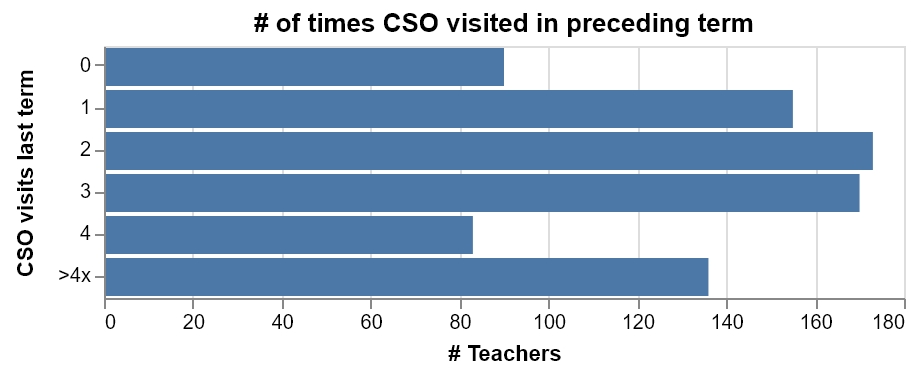
\includegraphics{../img/csovisct_ch.png}
\caption{CSO Visits}
\end{figure}

    We see that roughly 11\% of the respondents, while they'd been visited
by a CSO in the past, had not been visited in the preceding term.
However, roughly 64\% of the respondents were visited between once per
term and once per month. Roughly 28\% of the teachers were visited by
their CSOs more frequently than monthly.

    \hypertarget{csos-activities-during-last-coaching-visit}{%
\subsubsection{CSOs' activities during last coaching
visit}\label{csos-activities-during-last-coaching-visit}}

We are interested in knowing what CSOs are focusing on when they pay a
visit to a school. Are they observing a lesson? Are they giving feedback
to the teacher? Do they assess pupils' fluency rates? Do they take
advantage of their presence at the school to meet with the head teacher
(HT)? What kinds of things are they doing \emph{besides} these
activities?

    \begin{Verbatim}[commandchars=\\\{\}]
{\color{incolor}In [{\color{incolor}7}]:} \PY{c+c1}{\PYZsh{} Generating table of CSOs\PYZsq{} activities during visits}
        \PY{n}{visact\PYZus{}df} \PY{o}{=} \PY{n}{pd}\PY{o}{.}\PY{n}{DataFrame}\PY{o}{.}\PY{n}{from\PYZus{}dict}\PY{p}{(}\PY{p}{\PYZob{}}\PY{l+s+s2}{\PYZdq{}}\PY{l+s+s2}{activities}\PY{l+s+s2}{\PYZdq{}}\PY{p}{:} \PY{p}{[}\PY{l+s+s2}{\PYZdq{}}\PY{l+s+s2}{Assessed pupils}\PY{l+s+s2}{\PYZdq{}}\PY{p}{,}
                                                           \PY{l+s+s2}{\PYZdq{}}\PY{l+s+s2}{Talked to HT}\PY{l+s+s2}{\PYZdq{}}\PY{p}{,}
                                                           \PY{l+s+s2}{\PYZdq{}}\PY{l+s+s2}{Provided feedback on lesson}\PY{l+s+s2}{\PYZdq{}}\PY{p}{,}
                                                           \PY{l+s+s2}{\PYZdq{}}\PY{l+s+s2}{Had general talk}\PY{l+s+s2}{\PYZdq{}}\PY{p}{,}
                                                           \PY{l+s+s2}{\PYZdq{}}\PY{l+s+s2}{Other}\PY{l+s+s2}{\PYZdq{}}\PY{p}{]}\PY{p}{,}
                                            \PY{l+s+s2}{\PYZdq{}}\PY{l+s+s2}{tchrs\PYZus{}reporting}\PY{l+s+s2}{\PYZdq{}}\PY{p}{:} \PY{p}{[}\PY{n}{tchrs}\PY{p}{[}\PY{n}{tchrs}\PY{o}{.}\PY{n}{vis\PYZus{}before} \PY{o}{!=} \PY{l+m+mi}{0}\PY{p}{]}\PY{o}{.}\PY{n}{vis\PYZus{}act\PYZus{}kids}\PY{o}{.}\PY{n}{sum}\PY{p}{(}\PY{p}{)}\PY{p}{,}
                                                                \PY{n}{tchrs}\PY{p}{[}\PY{n}{tchrs}\PY{o}{.}\PY{n}{vis\PYZus{}before} \PY{o}{!=} \PY{l+m+mi}{0}\PY{p}{]}\PY{o}{.}\PY{n}{vis\PYZus{}act\PYZus{}ht}\PY{o}{.}\PY{n}{sum}\PY{p}{(}\PY{p}{)}\PY{p}{,}
                                                                \PY{n}{tchrs}\PY{p}{[}\PY{n}{tchrs}\PY{o}{.}\PY{n}{vis\PYZus{}before} \PY{o}{!=} \PY{l+m+mi}{0}\PY{p}{]}\PY{o}{.}\PY{n}{vis\PYZus{}act\PYZus{}fdbk}\PY{o}{.}\PY{n}{sum}\PY{p}{(}\PY{p}{)}\PY{p}{,}
                                                                \PY{n}{tchrs}\PY{p}{[}\PY{n}{tchrs}\PY{o}{.}\PY{n}{vis\PYZus{}before} \PY{o}{!=} \PY{l+m+mi}{0}\PY{p}{]}\PY{o}{.}\PY{n}{vis\PYZus{}act\PYZus{}gen}\PY{o}{.}\PY{n}{sum}\PY{p}{(}\PY{p}{)}\PY{p}{,}
                                                                \PY{n}{tchrs}\PY{p}{[}\PY{n}{tchrs}\PY{o}{.}\PY{n}{vis\PYZus{}before} \PY{o}{!=} \PY{l+m+mi}{0}\PY{p}{]}\PY{o}{.}\PY{n}{vis\PYZus{}act\PYZus{}other}\PY{o}{.}\PY{n}{sum}\PY{p}{(}\PY{p}{)}\PY{p}{]}\PY{p}{\PYZcb{}}\PY{p}{)}
        \PY{n}{visact\PYZus{}df}\PY{p}{[}\PY{l+s+s2}{\PYZdq{}}\PY{l+s+s2}{pct}\PY{l+s+s2}{\PYZdq{}}\PY{p}{]} \PY{o}{=} \PY{n}{np}\PY{o}{.}\PY{n}{round}\PY{p}{(}\PY{n}{visact\PYZus{}df}\PY{o}{.}\PY{n}{tchrs\PYZus{}reporting}\PY{o}{.}\PY{n}{apply}\PY{p}{(}\PY{k}{lambda} \PY{n}{x}\PY{p}{:} \PY{l+m+mi}{100} \PY{o}{*} \PY{p}{(}\PY{n}{x}\PY{o}{/}\PY{p}{(}\PY{n}{tchr\PYZus{}ct} \PY{o}{\PYZhy{}} \PY{n}{never}\PY{p}{)}\PY{p}{)}\PY{p}{)}\PY{p}{,} \PY{n}{decimals}\PY{o}{=}\PY{l+m+mi}{2}\PY{p}{)}
        \PY{n}{visact\PYZus{}df}
\end{Verbatim}

\begin{Verbatim}[commandchars=\\\{\}]
{\color{outcolor}Out[{\color{outcolor}7}]:}                     activities  tchrs\_reporting    pct
        0  Assessed pupils              688              83.84
        1  Talked to HT                 516              62.88
        2  Provided feedback on lesson  734              89.44
        3  Had general talk             364              44.36
        4  Other                        127              15.48
\end{Verbatim}
            
    \begin{Verbatim}[commandchars=\\\{\}]
{\color{incolor}In [{\color{incolor}8}]:} \PY{c+c1}{\PYZsh{} Generating the graph of CSOs\PYZsq{} activities during the previous visit}
        \PY{n}{csoprevvis\PYZus{}ch} \PY{o}{=} \PY{n}{alt}\PY{o}{.}\PY{n}{Chart}\PY{p}{(}\PY{n}{visact\PYZus{}df}\PY{p}{,} \PY{n}{title}\PY{o}{=}\PY{l+s+s2}{\PYZdq{}}\PY{l+s+s2}{CSO activities during previous visit}\PY{l+s+s2}{\PYZdq{}}\PY{p}{)}\PY{o}{.}\PY{n}{mark\PYZus{}bar}\PY{p}{(}\PY{p}{)}\PY{o}{.}\PY{n}{encode}\PY{p}{(}
        \PY{n}{alt}\PY{o}{.}\PY{n}{Y}\PY{p}{(}\PY{l+s+s2}{\PYZdq{}}\PY{l+s+s2}{activities:O}\PY{l+s+s2}{\PYZdq{}}\PY{p}{,} 
              \PY{n}{title}\PY{o}{=}\PY{l+s+s2}{\PYZdq{}}\PY{l+s+s2}{Activities named}\PY{l+s+s2}{\PYZdq{}}\PY{p}{,}
              \PY{n}{sort} \PY{o}{=} \PY{n}{alt}\PY{o}{.}\PY{n}{EncodingSortField}\PY{p}{(}\PY{n}{field}\PY{o}{=}\PY{l+s+s2}{\PYZdq{}}\PY{l+s+s2}{tchrs\PYZus{}reporting}\PY{l+s+s2}{\PYZdq{}}\PY{p}{,} \PY{n}{op}\PY{o}{=}\PY{l+s+s2}{\PYZdq{}}\PY{l+s+s2}{values}\PY{l+s+s2}{\PYZdq{}}\PY{p}{,} \PY{n}{order}\PY{o}{=}\PY{l+s+s2}{\PYZdq{}}\PY{l+s+s2}{ascending}\PY{l+s+s2}{\PYZdq{}}\PY{p}{)}\PY{p}{)}\PY{p}{,}
        \PY{n}{alt}\PY{o}{.}\PY{n}{X}\PY{p}{(}\PY{l+s+s2}{\PYZdq{}}\PY{l+s+s2}{pct:Q}\PY{l+s+s2}{\PYZdq{}}\PY{p}{,}
              \PY{n}{title}\PY{o}{=}\PY{l+s+s2}{\PYZdq{}}\PY{l+s+si}{\PYZpc{} o}\PY{l+s+s2}{f teachers responding}\PY{l+s+s2}{\PYZdq{}}\PY{p}{)}\PY{p}{,}
        \PY{n}{tooltip} \PY{o}{=} \PY{l+s+s2}{\PYZdq{}}\PY{l+s+s2}{tchrs\PYZus{}reporting}\PY{l+s+s2}{\PYZdq{}}\PY{p}{)}
        \PY{n}{csoprevvis\PYZus{}ch}\PY{o}{.}\PY{n}{save}\PY{p}{(}\PY{l+s+s2}{\PYZdq{}}\PY{l+s+s2}{../img/csoprevvis\PYZus{}ch.png}\PY{l+s+s2}{\PYZdq{}}\PY{p}{,} \PY{n}{scale\PYZus{}factor}\PY{o}{=}\PY{l+m+mf}{2.0}\PY{p}{)}
\end{Verbatim}

    \begin{figure}
\centering
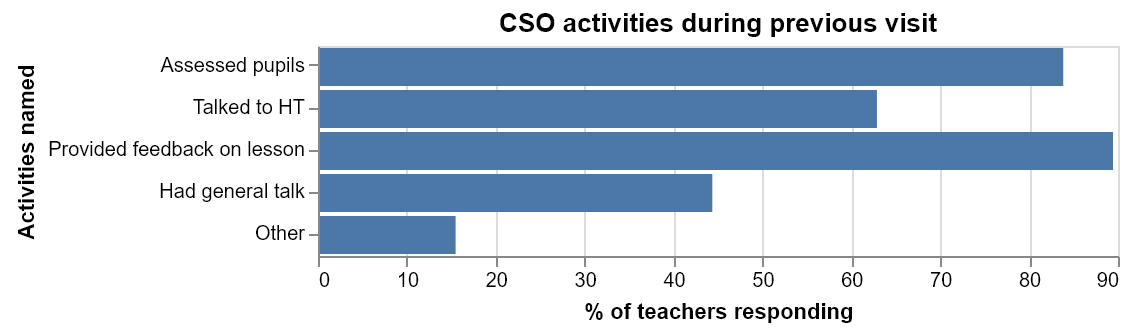
\includegraphics{../img/csoprevvis_ch.png}
\caption{CSOs' Activities}
\end{figure}

    Nearly 90\% of teachers report that when the CSO last visited, s/he
provided feedback on a lesson. A fairly comparable proportion said that
the CSO assessed pupils. Neither of these is surprising, as those
activities are key features of a ``reimbursable'' or ``valid'' lesson
observation. If anything, it is interesting that these numbers are not
higher, given that we have excluded from our denominator those teachers
who said they had never received a visit from the CSO.

Of note is the relatively low proportion of teachers reporting the CSO
had spoken with the HT. While Tusome encourages CSOs to speak with HTs
as part of the standard protocol for visiting a school, it is not
explicitly considered as a factor for reimbursement of transportation
costs for visiting that school.

That said, it is also possible that teachers may simply not be aware of
activities taking place outside of their classroom. They and their
classrooms would have been the objects of the lesson observation and
fluency assessment; they may not have as much visibility into what
happened before or after the CSO entered their classroom.

A little over 15\% of teachers reported the CSO conducted an activity
that was not listed in the questionnaire. Below we have sampled 20 of
the things that they reported which were not captured in the
questionnaire.

    \begin{Verbatim}[commandchars=\\\{\}]
{\color{incolor}In [{\color{incolor}9}]:} \PY{c+c1}{\PYZsh{} Generating a list of the \PYZsq{}other\PYZsq{} activities CSOs did when visiting}
        \PY{n+nb}{print}\PY{p}{(}\PY{n}{tchrs}\PY{p}{[}\PY{n}{tchrs}\PY{o}{.}\PY{n}{vis\PYZus{}act\PYZus{}other\PYZus{}det}\PY{o}{.}\PY{n}{notna}\PY{p}{(}\PY{p}{)} \PY{o}{\PYZam{}} \PY{p}{(}\PY{n}{tchrs}\PY{o}{.}\PY{n}{vis\PYZus{}act\PYZus{}other\PYZus{}det} \PY{o}{!=} \PY{l+s+s2}{\PYZdq{}}\PY{l+s+s2}{\PYZdq{}}\PY{p}{)}\PY{p}{]}\PY{o}{.}\PY{n}{vis\PYZus{}act\PYZus{}other\PYZus{}det}\PY{o}{.}\PY{n}{sample}\PY{p}{(}\PY{l+m+mi}{20}\PY{p}{)}\PY{p}{)}
\end{Verbatim}

    \begin{Verbatim}[commandchars=\\\{\}]
384    She talked to other teachers about Tusome .She said Tusome should not be taken as program for grade 1 to 3 only but an intervention that all the teachers in the school should be compliant with.
736    He asked for the lesson i was teaching ,he sat at the back of the class and observed my lesson as I taught. After the lesson he assessed three learners and gave me feedback                     
95     I present the lesson as she observes the lesson                                                                                                                                                  
619    The CSO observes me teach,after the lessons I sit with her to discuss what I did well and then she explains to me what I did not do well.She explains or modelles how I should have don e it.    
268    CSO checks all my professional documents                                                                                                                                                         
399    He always telles us through the Ht about his coming .He picks 3 pupils for assessment then we sit to evaluate the lesson starting with what went well and areas of improvement.                  
729    The CSO observed my lesson ,assessed three learners ,gave me feedback and advised me regarding covering Tusome books                                                                             
154    Once attended the parents meeting and went with my class performance data to present to parents i felt good since my pupils had read fluently                                                    
525    The CSO first meets with all the teachers and plan how the classroom support visits shall be for all the teachers.                                                                               
325    He observed lesson,he gave me feedback on areas of improvement                                                                                                                                   
2      requests me to prepare for the lesson in adavnace and details of the lesson, boys and girls                                                                                                      
687    Cover the pupils' books                                                                                                                                                                          
659    She assembled all lower Primary teachers and advised us on how to teach successful lessons.                                                                                                      
300    He sought information on book shortages and resources such as letter cards                                                                                                                       
208    Helped me on how to use the teachers guide because I was new to the system.                                                                                                                      
752    I saw him sit at the back,he checked pupils work and he checked pupils books                                                                                                                     
401    He spoke to headteacher,observed my class,assessed pupils and gave me feed back on my class                                                                                                      
721    assesed children,spoke to head teacher and gave me feedback                                                                                                                                      
730    The CSO observed my lessons (English,Kiswahili \& Maths and gives me feedback on areas of improvement                                                                                             
648    guidance on preparation of teacher documentation                                                                                                                                                 
Name: vis\_act\_other\_det, dtype: object

    \end{Verbatim}

    \hypertarget{csos-using-tablets-or-pen-paper-during-observation}{%
\subsubsection{CSOs using tablets or pen \& paper during
observation}\label{csos-using-tablets-or-pen-paper-during-observation}}

The \emph{Tangerine:Tutor} app was developed with the intent and belief
that CSOs would use it \emph{while observing} the lesson. However,
Tusome staff report that not all CSOs find the tablet interface
comfortable, and not all use it with ease. So we asked teachers to
report whether CSOs use the tablets during the lesson observation, and
also whether they use pen and paper.

    Roughly 90\% of teachers reported that the CSOs use tablets during
lesson observation; roughly 81\% of teachers reported the CSOs use pen
and paper during the lesson observation.

    \begin{Verbatim}[commandchars=\\\{\}]
{\color{incolor}In [{\color{incolor}10}]:} \PY{c+c1}{\PYZsh{} Generating the table about usage of tablets and pencils}
         \PY{n}{tabs\PYZus{}n\PYZus{}pencils} \PY{o}{=} \PY{n}{pd}\PY{o}{.}\PY{n}{crosstab}\PY{p}{(}\PY{n}{tchrs}\PY{o}{.}\PY{n}{cso\PYZus{}usetab\PYZus{}yn}\PY{p}{,} \PY{n}{tchrs}\PY{o}{.}\PY{n}{cso\PYZus{}usepcl\PYZus{}yn}\PY{p}{)}
         \PY{n}{tabs\PYZus{}n\PYZus{}pencils} \PY{o}{=} \PY{n}{tabs\PYZus{}n\PYZus{}pencils}\PY{o}{.}\PY{n}{rename\PYZus{}axis}\PY{p}{(}\PY{l+s+s2}{\PYZdq{}}\PY{l+s+s2}{Uses tablet}\PY{l+s+s2}{\PYZdq{}}\PY{p}{)}\PY{o}{.}\PY{n}{rename\PYZus{}axis}\PY{p}{(}\PY{l+s+s2}{\PYZdq{}}\PY{l+s+s2}{Uses pen and paper}\PY{l+s+s2}{\PYZdq{}}\PY{p}{,} \PY{n}{axis}\PY{o}{=}\PY{l+s+s2}{\PYZdq{}}\PY{l+s+s2}{columns}\PY{l+s+s2}{\PYZdq{}}\PY{p}{)}
         \PY{n}{tabs\PYZus{}n\PYZus{}pencils} \PY{o}{=} \PY{n}{tabs\PYZus{}n\PYZus{}pencils}\PY{o}{.}\PY{n}{rename}\PY{p}{(}\PY{p}{\PYZob{}}\PY{l+m+mi}{0}\PY{p}{:} \PY{l+s+s2}{\PYZdq{}}\PY{l+s+s2}{No}\PY{l+s+s2}{\PYZdq{}}\PY{p}{,} \PY{l+m+mi}{1}\PY{p}{:} \PY{l+s+s2}{\PYZdq{}}\PY{l+s+s2}{Yes}\PY{l+s+s2}{\PYZdq{}}\PY{p}{\PYZcb{}}\PY{p}{,} \PY{n}{axis}\PY{o}{=}\PY{l+s+s2}{\PYZdq{}}\PY{l+s+s2}{columns}\PY{l+s+s2}{\PYZdq{}}\PY{p}{)}\PY{o}{.}\PY{n}{rename}\PY{p}{(}\PY{p}{\PYZob{}}\PY{l+m+mi}{0}\PY{p}{:} \PY{l+s+s2}{\PYZdq{}}\PY{l+s+s2}{No}\PY{l+s+s2}{\PYZdq{}}\PY{p}{,} \PY{l+m+mi}{1}\PY{p}{:} \PY{l+s+s2}{\PYZdq{}}\PY{l+s+s2}{Yes}\PY{l+s+s2}{\PYZdq{}}\PY{p}{\PYZcb{}}\PY{p}{,} \PY{n}{axis}\PY{o}{=}\PY{l+s+s2}{\PYZdq{}}\PY{l+s+s2}{index}\PY{l+s+s2}{\PYZdq{}}\PY{p}{)}
         \PY{n}{tabs\PYZus{}n\PYZus{}pencils}
\end{Verbatim}

\begin{Verbatim}[commandchars=\\\{\}]
{\color{outcolor}Out[{\color{outcolor}10}]:} Uses pen and paper  No  Yes
         Uses tablet                
         No                  3   17 
         Yes                 72  657
\end{Verbatim}
            
    We see that the overwhelming majority of CSOs are using both tablets
\emph{and} pen-and-paper systems when observing the teachers' lesson.
There have historically been some instruments/data that CSOs were tasked
by TSC to complete that were not rendered in \emph{Tangerine} format on
the tablets; as of midway through Term 3 of the 2018 academic year,
those instruments (mostly for the TSC's TPAD {[}Teacher Performance
Appraisal and Development{]} project) are now in \emph{Tangerine}. While
the use of pen and paper does not appear to have come at the expense of
using the tablets - indeed, it appears to be complementary, as nearly
all CSOs are using both - Tusome should nonetheless follow up on these
reports of CSOs' usage of pen and paper to understand the roots of the
practice.

    \hypertarget{csos-usage-of-the-tablets-to-assess-pupils-performance}{%
\subsubsection{CSOs' usage of the tablets to assess pupils'
performance}\label{csos-usage-of-the-tablets-to-assess-pupils-performance}}

Tusome's coaching protocol requires CSOs to randomly select three
children from the classroom at the end of the lesson to assess their
reading fluency. The prompt the children are to read from is a laminated
sheet of paper with a short passage printed on it; the CSOs are
instructed to use the tablet to record the children's responses. The
tablet is then able to calculate fluency rates and store those as data
associated with that observation.

Approximately 88\% of the teachers reported that CSOs use the tablets to
assess children's reading fluency.

    \hypertarget{teachers-experience-of-feedback-and-csos-use-of-tablets-during-feedback}{%
\subsubsection{Teachers' experience of feedback, and CSOs' use of
tablets during
feedback}\label{teachers-experience-of-feedback-and-csos-use-of-tablets-during-feedback}}

Tusome asked teachers whether the CSO gave feedback on the lesson last
time s/he paid a visit, whether s/he used the tablet to do so, and
whether the teacher was able to recall specific feedback the CSO
provided.

    \begin{Verbatim}[commandchars=\\\{\}]
{\color{incolor}In [{\color{incolor}11}]:} \PY{c+c1}{\PYZsh{} Generating table of CSO use of tablets for feedback}
         \PY{n}{feedback} \PY{o}{=} \PY{p}{\PYZob{}}\PY{l+s+s2}{\PYZdq{}}\PY{l+s+s2}{CSO gave feedback}\PY{l+s+s2}{\PYZdq{}}\PY{p}{:} \PY{n}{tchrs}\PY{o}{.}\PY{n}{cso\PYZus{}gave\PYZus{}fdbk\PYZus{}yn}\PY{o}{.}\PY{n}{sum}\PY{p}{(}\PY{p}{)}\PY{p}{,}
                     \PY{l+s+s2}{\PYZdq{}}\PY{l+s+s2}{CSO used a tablet for feedback}\PY{l+s+s2}{\PYZdq{}}\PY{p}{:} \PY{n}{tchrs}\PY{o}{.}\PY{n}{cso\PYZus{}usetab\PYZus{}fdbk\PYZus{}yn}\PY{o}{.}\PY{n}{sum}\PY{p}{(}\PY{p}{)}\PY{p}{,}
                     \PY{l+s+s2}{\PYZdq{}}\PY{l+s+s2}{Tchr remembers feedback}\PY{l+s+s2}{\PYZdq{}}\PY{p}{:} \PY{n}{tchrs}\PY{o}{.}\PY{n}{cso\PYZus{}fdbk\PYZus{}remember}\PY{o}{.}\PY{n}{sum}\PY{p}{(}\PY{p}{)}\PY{p}{\PYZcb{}}
         \PY{n}{fdbk\PYZus{}df} \PY{o}{=} \PY{n}{pd}\PY{o}{.}\PY{n}{DataFrame}\PY{o}{.}\PY{n}{from\PYZus{}dict}\PY{p}{(}\PY{n}{feedback}\PY{p}{,} \PY{n}{orient}\PY{o}{=}\PY{l+s+s2}{\PYZdq{}}\PY{l+s+s2}{index}\PY{l+s+s2}{\PYZdq{}}\PY{p}{,} \PY{n}{columns}\PY{o}{=}\PY{p}{[}\PY{l+s+s2}{\PYZdq{}}\PY{l+s+s2}{ct}\PY{l+s+s2}{\PYZdq{}}\PY{p}{]}\PY{p}{)}
         \PY{n}{fdbk\PYZus{}df}\PY{p}{[}\PY{l+s+s2}{\PYZdq{}}\PY{l+s+s2}{pct}\PY{l+s+s2}{\PYZdq{}}\PY{p}{]} \PY{o}{=} \PY{l+m+mi}{100} \PY{o}{*} \PY{n}{np}\PY{o}{.}\PY{n}{round}\PY{p}{(}\PY{n}{fdbk\PYZus{}df}\PY{p}{[}\PY{l+s+s2}{\PYZdq{}}\PY{l+s+s2}{ct}\PY{l+s+s2}{\PYZdq{}}\PY{p}{]} \PY{o}{/} \PY{n}{tchrs}\PY{o}{.}\PY{n}{shape}\PY{p}{[}\PY{l+m+mi}{0}\PY{p}{]}\PY{p}{,} \PY{n}{decimals}\PY{o}{=}\PY{l+m+mi}{3}\PY{p}{)}
         \PY{n}{fdbk\PYZus{}df} \PY{o}{=} \PY{n}{fdbk\PYZus{}df}\PY{o}{.}\PY{n}{rename\PYZus{}axis}\PY{p}{(}\PY{l+s+s2}{\PYZdq{}}\PY{l+s+s2}{event}\PY{l+s+s2}{\PYZdq{}}\PY{p}{)}\PY{o}{.}\PY{n}{reset\PYZus{}index}\PY{p}{(}\PY{p}{)}
         \PY{n}{fdbk\PYZus{}df}
\end{Verbatim}

\begin{Verbatim}[commandchars=\\\{\}]
{\color{outcolor}Out[{\color{outcolor}11}]:}                             event     ct   pct
         0  CSO gave feedback               757.0  91.4
         1  CSO used a tablet for feedback  676.0  81.6
         2  Tchr remembers feedback         725.0  87.6
\end{Verbatim}
            
    Below we have sampled 20 of the things that they reported which were not
captured in the questionnaire.

    \begin{Verbatim}[commandchars=\\\{\}]
{\color{incolor}In [{\color{incolor}12}]:} \PY{c+c1}{\PYZsh{} Sample of details regarding the details of feedback CSOs provided}
         \PY{n+nb}{print}\PY{p}{(}\PY{n}{tchrs}\PY{p}{[}\PY{n}{tchrs}\PY{o}{.}\PY{n}{cso\PYZus{}fdbk\PYZus{}det}\PY{o}{.}\PY{n}{notna}\PY{p}{(}\PY{p}{)} \PY{o}{\PYZam{}} \PY{p}{(}\PY{n}{tchrs}\PY{o}{.}\PY{n}{cso\PYZus{}fdbk\PYZus{}det} \PY{o}{!=} \PY{l+s+s2}{\PYZdq{}}\PY{l+s+s2}{\PYZdq{}}\PY{p}{)}\PY{p}{]}\PY{o}{.}\PY{n}{cso\PYZus{}fdbk\PYZus{}det}\PY{o}{.}\PY{n}{sample}\PY{p}{(}\PY{l+m+mi}{20}\PY{p}{)}\PY{p}{)}
\end{Verbatim}

    \begin{Verbatim}[commandchars=\\\{\}]
650    Advice to use correct speed to the learners. How to group slow learners                                                                                                                  
58     He asked me to cover all Tusome books .He also told me to keep time and limit lessons to 30 minutes                                                                                      
622    I was appreciated on time management and advised me to support non readers                                                                                                               
778    To avoid using other languages in an english lesson but to use teaching aids to explain meanings.                                                                                        
273    I took a lot of time in teaching, CSO told me to maintain perky pace. He told me my pupils are good.                                                                                     
652    Improve in pronunciation of sounds                                                                                                                                                       
686    create time and help slow learners in word blending                                                                                                                                      
62     CSO told me the lesson was Ok, I was advised that pupils to read the story fluently                                                                                                      
186    He told me am able to follow the Tusome steps of I do, We do, You do but in some areas am too fast. He also told me that a majority of my learners are able to read.                     
183    He told me am improving and if I continue that way me children will be the best in the zone.                                                                                             
529    during sentence construction i should chose few pupils to give                                                                                                                           
668    The CSO guided on how to teach using the DIM and corrected me on the 'we do'.                                                                                                            
380    he told me to improve my friendship with the learners and help them to be courageous                                                                                                     
397    From the results of reading fluency compared to the previous vist I have observed improvement. Keep supporting the slow learners.                                                        
431    We discuscussed ORF- " I was told to ensure all pupils in my class are able to read as per the expected benchmark level                                                                  
760    The CSO used the tablet to play for me the sounds that I had difficulty in pronouncing                                                                                                   
748    He commented on time taken during the lesson and how to improve on direct instruction model                                                                                              
204    The CSO observed that the pupils were not reading at the benchmark                                                                                                                       
638    The CSO told me i was audible enough, I had good pronounciation of the sounds, the learners were well involved in the lesson, he said i infused the CBC and I had good class management..
267    She showed me the number of words read by selected pupils during assessment                                                                                                              
Name: cso\_fdbk\_det, dtype: object

    \end{Verbatim}

    The tablets come equipped with various aids that CSOs could use to help
coach teachers. In addition to the contents of the auto-generated
feedback, CSOs could use the \emph{Papaya} application to model
pronunciation of letter sounds, the videos demonstrating effective
lesson delivery, etc. Of the teachers reporting CSOs provided feedback
of some kind, 56\% indicated that the CSO showed them something directly
on the tablet.

    \begin{Verbatim}[commandchars=\\\{\}]
{\color{incolor}In [{\color{incolor}13}]:} \PY{c+c1}{\PYZsh{} Generating dataframe of feedback shown by CSOs to teachers}
         \PY{n}{fdbk\PYZus{}shown\PYZus{}df} \PY{o}{=} \PY{n}{pd}\PY{o}{.}\PY{n}{DataFrame}\PY{o}{.}\PY{n}{from\PYZus{}dict}\PY{p}{(}\PY{p}{\PYZob{}}\PY{l+s+s2}{\PYZdq{}}\PY{l+s+s2}{resources}\PY{l+s+s2}{\PYZdq{}}\PY{p}{:} \PY{p}{[}\PY{l+s+s2}{\PYZdq{}}\PY{l+s+s2}{Tips from feedback screen}\PY{l+s+s2}{\PYZdq{}}\PY{p}{,}
                                                            \PY{l+s+s2}{\PYZdq{}}\PY{l+s+s2}{Pupils}\PY{l+s+s2}{\PYZsq{}}\PY{l+s+s2}{ reading fluency}\PY{l+s+s2}{\PYZdq{}}\PY{p}{,}
                                                            \PY{l+s+s2}{\PYZdq{}}\PY{l+s+s2}{Videos of lesson delivery}\PY{l+s+s2}{\PYZdq{}}\PY{p}{,}
                                                            \PY{l+s+s2}{\PYZdq{}}\PY{l+s+s2}{Letter sounds in Papaya}\PY{l+s+s2}{\PYZdq{}}\PY{p}{,}
                                                            \PY{l+s+s2}{\PYZdq{}}\PY{l+s+s2}{Other}\PY{l+s+s2}{\PYZdq{}}\PY{p}{]}\PY{p}{,}
                                             \PY{l+s+s2}{\PYZdq{}}\PY{l+s+s2}{tchrs\PYZus{}reporting}\PY{l+s+s2}{\PYZdq{}}\PY{p}{:}\PY{p}{[}
                                                 \PY{n}{tchrs}\PY{p}{[}\PY{n}{tchrs}\PY{o}{.}\PY{n}{vis\PYZus{}act\PYZus{}fdbk} \PY{o}{!=} \PY{l+m+mi}{0}\PY{p}{]}\PY{o}{.}\PY{n}{cso\PYZus{}shw\PYZus{}tips}\PY{o}{.}\PY{n}{sum}\PY{p}{(}\PY{p}{)}\PY{p}{,}
                                                 \PY{n}{tchrs}\PY{p}{[}\PY{n}{tchrs}\PY{o}{.}\PY{n}{vis\PYZus{}act\PYZus{}fdbk} \PY{o}{!=} \PY{l+m+mi}{0}\PY{p}{]}\PY{o}{.}\PY{n}{cso\PYZus{}shw\PYZus{}fluency}\PY{o}{.}\PY{n}{sum}\PY{p}{(}\PY{p}{)}\PY{p}{,}
                                                 \PY{n}{tchrs}\PY{p}{[}\PY{n}{tchrs}\PY{o}{.}\PY{n}{vis\PYZus{}act\PYZus{}fdbk} \PY{o}{!=} \PY{l+m+mi}{0}\PY{p}{]}\PY{o}{.}\PY{n}{cso\PYZus{}shw\PYZus{}video}\PY{o}{.}\PY{n}{sum}\PY{p}{(}\PY{p}{)}\PY{p}{,}
                                                 \PY{n}{tchrs}\PY{p}{[}\PY{n}{tchrs}\PY{o}{.}\PY{n}{vis\PYZus{}act\PYZus{}fdbk} \PY{o}{!=} \PY{l+m+mi}{0}\PY{p}{]}\PY{o}{.}\PY{n}{cso\PYZus{}shw\PYZus{}lsnd}\PY{o}{.}\PY{n}{sum}\PY{p}{(}\PY{p}{)}\PY{p}{,}
                                                 \PY{n}{tchrs}\PY{p}{[}\PY{n}{tchrs}\PY{o}{.}\PY{n}{vis\PYZus{}act\PYZus{}fdbk} \PY{o}{!=} \PY{l+m+mi}{0}\PY{p}{]}\PY{o}{.}\PY{n}{cso\PYZus{}shw\PYZus{}other}\PY{o}{.}\PY{n}{sum}\PY{p}{(}\PY{p}{)}\PY{p}{]}\PY{p}{\PYZcb{}}\PY{p}{)}
         \PY{n}{fdbk\PYZus{}shown\PYZus{}df}\PY{p}{[}\PY{l+s+s2}{\PYZdq{}}\PY{l+s+s2}{pct}\PY{l+s+s2}{\PYZdq{}}\PY{p}{]} \PY{o}{=} \PY{n}{np}\PY{o}{.}\PY{n}{round}\PY{p}{(}
             \PY{n}{fdbk\PYZus{}shown\PYZus{}df}\PY{o}{.}\PY{n}{tchrs\PYZus{}reporting}\PY{o}{.}\PY{n}{apply}\PY{p}{(}
             \PY{k}{lambda} \PY{n}{x}\PY{p}{:} \PY{l+m+mi}{100} \PY{o}{*} \PY{p}{(}\PY{n}{x}\PY{o}{/}\PY{n}{visact\PYZus{}df}\PY{p}{[}\PY{n}{visact\PYZus{}df}\PY{o}{.}\PY{n}{activities}\PY{o}{==}\PY{l+s+s2}{\PYZdq{}}\PY{l+s+s2}{Provided feedback on lesson}\PY{l+s+s2}{\PYZdq{}}\PY{p}{]}\PY{o}{.}\PY{n}{tchrs\PYZus{}reporting}\PY{p}{)}\PY{p}{)}\PY{p}{,}
             \PY{n}{decimals}\PY{o}{=}\PY{l+m+mi}{2}\PY{p}{)}
         \PY{n}{fdbk\PYZus{}shown\PYZus{}df}
\end{Verbatim}

\begin{Verbatim}[commandchars=\\\{\}]
{\color{outcolor}Out[{\color{outcolor}13}]:}                    resources  tchrs\_reporting    pct
         0  Tips from feedback screen  167              22.75
         1  Pupils' reading fluency    260              35.42
         2  Videos of lesson delivery  128              17.44
         3  Letter sounds in Papaya    230              31.34
         4  Other                      54               7.36 
\end{Verbatim}
            
    \begin{Verbatim}[commandchars=\\\{\}]
{\color{incolor}In [{\color{incolor}14}]:} \PY{c+c1}{\PYZsh{} Generating chart of tablet\PYZhy{}based resources shown to teachers}
         \PY{n}{tabres\PYZus{}ch} \PY{o}{=} \PY{n}{alt}\PY{o}{.}\PY{n}{Chart}\PY{p}{(}\PY{n}{fdbk\PYZus{}shown\PYZus{}df}\PY{p}{,} \PY{n}{title}\PY{o}{=}\PY{l+s+s2}{\PYZdq{}}\PY{l+s+s2}{Tablet\PYZhy{}based resources shown to Teachers by CSOs}\PY{l+s+s2}{\PYZdq{}}\PY{p}{)}\PY{o}{.}\PY{n}{mark\PYZus{}bar}\PY{p}{(}\PY{p}{)}\PY{o}{.}\PY{n}{encode}\PY{p}{(}
         \PY{n}{alt}\PY{o}{.}\PY{n}{Y}\PY{p}{(}\PY{l+s+s2}{\PYZdq{}}\PY{l+s+s2}{resources:O}\PY{l+s+s2}{\PYZdq{}}\PY{p}{,} 
               \PY{n}{title}\PY{o}{=}\PY{l+s+s2}{\PYZdq{}}\PY{l+s+s2}{Resources named}\PY{l+s+s2}{\PYZdq{}}\PY{p}{,}
               \PY{n}{sort} \PY{o}{=} \PY{n}{alt}\PY{o}{.}\PY{n}{EncodingSortField}\PY{p}{(}\PY{n}{field}\PY{o}{=}\PY{l+s+s2}{\PYZdq{}}\PY{l+s+s2}{tchrs\PYZus{}reporting}\PY{l+s+s2}{\PYZdq{}}\PY{p}{,} \PY{n}{op}\PY{o}{=}\PY{l+s+s2}{\PYZdq{}}\PY{l+s+s2}{values}\PY{l+s+s2}{\PYZdq{}}\PY{p}{,} \PY{n}{order}\PY{o}{=}\PY{l+s+s2}{\PYZdq{}}\PY{l+s+s2}{ascending}\PY{l+s+s2}{\PYZdq{}}\PY{p}{)}\PY{p}{)}\PY{p}{,}
         \PY{n}{alt}\PY{o}{.}\PY{n}{X}\PY{p}{(}\PY{l+s+s2}{\PYZdq{}}\PY{l+s+s2}{pct:Q}\PY{l+s+s2}{\PYZdq{}}\PY{p}{,}
               \PY{n}{title}\PY{o}{=}\PY{l+s+s2}{\PYZdq{}}\PY{l+s+si}{\PYZpc{} o}\PY{l+s+s2}{f teachers responding}\PY{l+s+s2}{\PYZdq{}}\PY{p}{)}\PY{p}{,}
         \PY{n}{tooltip} \PY{o}{=} \PY{l+s+s2}{\PYZdq{}}\PY{l+s+s2}{tchrs\PYZus{}reporting}\PY{l+s+s2}{\PYZdq{}}\PY{p}{)}
         \PY{n}{tabres\PYZus{}ch}\PY{o}{.}\PY{n}{save}\PY{p}{(}\PY{l+s+s2}{\PYZdq{}}\PY{l+s+s2}{../img/tabres\PYZus{}ch.png}\PY{l+s+s2}{\PYZdq{}}\PY{p}{,} \PY{n}{scale\PYZus{}factor}\PY{o}{=}\PY{l+m+mf}{2.0}\PY{p}{)}
\end{Verbatim}

    \begin{figure}
\centering
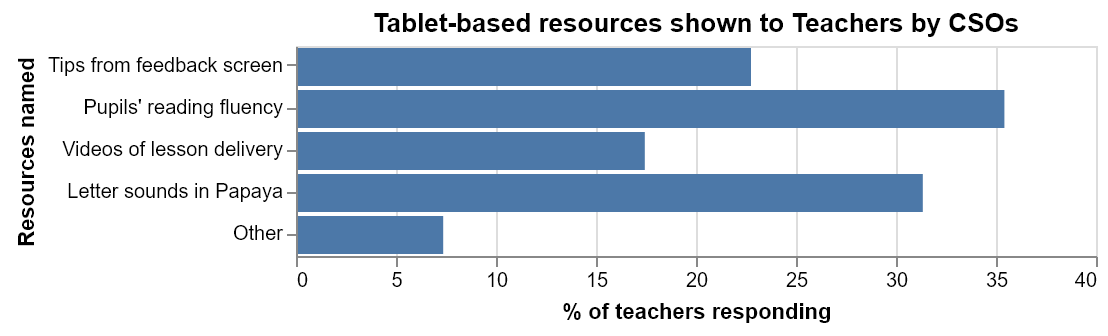
\includegraphics{../img/tabres_ch.png}
\caption{Tablet Resources Chart}
\end{figure}

    Overall, fewer than 50\% of teachers indicated that CSOs showed them
something on the tablet as part of the feedback session. Where the CSO
showed something to the teacher, it was most frequently pupils' reading
fluency (at 35\%), with Papaya letter sounds the next most common (at
31\%).

    \textbf{N.B.}: { Update cell w literate programming re: which activity
is in the lead. (Abstract one level further.)}

Below we have sampled 20 of the things that they reported which were not
captured in the questionnaire.

    \begin{Verbatim}[commandchars=\\\{\}]
{\color{incolor}In [{\color{incolor}15}]:} \PY{c+c1}{\PYZsh{} Printing sample of teachers\PYZsq{} feedback re: things CSOs showed them on the tablet}
         \PY{n+nb}{print}\PY{p}{(}\PY{n}{tchrs}\PY{p}{[}\PY{n}{tchrs}\PY{o}{.}\PY{n}{cso\PYZus{}shw\PYZus{}other\PYZus{}det}\PY{o}{.}\PY{n}{notna}\PY{p}{(}\PY{p}{)} \PY{o}{\PYZam{}} \PY{p}{(}\PY{n}{tchrs}\PY{o}{.}\PY{n}{cso\PYZus{}shw\PYZus{}other\PYZus{}det} \PY{o}{!=} \PY{l+s+s2}{\PYZdq{}}\PY{l+s+s2}{\PYZdq{}}\PY{p}{)}\PY{p}{]}\PY{o}{.}\PY{n}{cso\PYZus{}shw\PYZus{}other\PYZus{}det}\PY{o}{.}\PY{n}{sample}\PY{p}{(}\PY{l+m+mi}{20}\PY{p}{)}\PY{p}{)}
\end{Verbatim}

    \begin{Verbatim}[commandchars=\\\{\}]
42     During training he showed us videos from the tablet                                                                         
720    Downloaded the letter sounds on my smart phone                                                                              
546    pronounciation of a word in the dictionary                                                                                  
506    He only showed us during the training                                                                                       
480    pronounciation of a word in the dictionary                                                                                  
106    Installed Papaya application in phones during trainings which I use whenever I had challenge in letter sounds.              
467    After the lesson is over he shows me the reading outcomes.                                                                  
369    he showed me the text which the pupils read during the pupils assessmenet                                                   
224    He showed me the words that were read incorrectly by the three learners that were selected to read on the stimulus          
781    The CSO showed me the feedback comments                                                                                     
447    The pupils assessment reading and how the tool counts the average number of words read by the pupils                        
127    Time management- The time I took to conduct the lesson                                                                      
577    the feedback on the tablet                                                                                                  
549    pronounciation of a word in the dictionary                                                                                  
785    I was shown the time the lesson took                                                                                        
614    The CSO ocassionally shows me pupils fluency rates and advises on how I should help the weak.                               
507    He only reads to me eg he reads the sections on how I needed to conduct the lesson or pupils reading outcome and time taken,
820    Mostly, I get the support from the head teacher who advises me on the areas i need to perform well                          
63     He showed me a video of a teacher teaching thumbs up/down                                                                   
514    He showed me a video of a teacher teaching silent blending                                                                  
Name: cso\_shw\_other\_det, dtype: object

    \end{Verbatim}

    \hypertarget{csos-use-of-feedback-visit-over-visit}{%
\subsubsection{CSOs' use of feedback
visit-over-visit}\label{csos-use-of-feedback-visit-over-visit}}

Tusome's theory of change stipulates that smaller, more frequent, and
more targeted coaching interactions will shift teacher behavior more
effectively than larger-scale, episodic training events that cover a
broad range of topics. This is the reason Tusome invests so heavily in
supporting CSOs to provide coaching support to teachers in the span
between large-scale training events.

Teachers, like most people, will be more likely to alter their behavior
if feedback is timely and consistent, and the teachers' response to it
is monitored rather than assumed. In this survey, roughly 63\% of
teachers indicated that when CSOs visited the school and observed the
teacher, they follow up on feedback from earlier visits.

    \textbf{T.D.}: { Update cells so definitions of variable
\texttt{literate\ programming} inputs are visible.}

    \hypertarget{teachers-self-reported-improvement-in-response-to-coaching}{%
\subsubsection{Teachers self-reported improvement in response to
coaching}\label{teachers-self-reported-improvement-in-response-to-coaching}}

Effectively measuring the quality of instruction or lesson delivery is a
very, very difficult task. (\textbf{T.D.}: { Provide citations, examples
of various approaches.})

The current study was not able to directly assess the quality of
teachers' lesson delivery, although Tusome is working on various other
studies which attempt to do so. However, we asked teachers whether they
felt the coaching received from CSOs had improved the quality of their
teaching. We first posed the question in regard to the teaching of
reading in Kiswahili and English, and then asked them whether the
coaching had improved their teaching in other subjects as well.

    \begin{Verbatim}[commandchars=\\\{\}]
{\color{incolor}In [{\color{incolor}16}]:} \PY{c+c1}{\PYZsh{} Generating dataframe of teacher\PYZsq{}s self\PYZhy{}reported improvement due to coaching}
         \PY{n}{better\PYZus{}tchr\PYZus{}df} \PY{o}{=} \PY{n}{pd}\PY{o}{.}\PY{n}{DataFrame}\PY{o}{.}\PY{n}{from\PYZus{}dict}\PY{p}{(}
             \PY{p}{\PYZob{}}\PY{l+s+s2}{\PYZdq{}}\PY{l+s+s2}{subject}\PY{l+s+s2}{\PYZdq{}}\PY{p}{:} \PY{p}{[}\PY{l+s+s2}{\PYZdq{}}\PY{l+s+s2}{Kiswahili \PYZam{} English reading}\PY{l+s+s2}{\PYZdq{}}\PY{p}{,}
                           \PY{l+s+s2}{\PYZdq{}}\PY{l+s+s2}{Other subjects}\PY{l+s+s2}{\PYZdq{}}\PY{p}{]}\PY{p}{,}
              \PY{l+s+s2}{\PYZdq{}}\PY{l+s+s2}{tchrs\PYZus{}reporting}\PY{l+s+s2}{\PYZdq{}}\PY{p}{:} \PY{p}{[}\PY{n}{tchrs}\PY{p}{[}\PY{p}{(}\PY{n}{tchrs}\PY{o}{.}\PY{n}{vis\PYZus{}act\PYZus{}fdbk} \PY{o}{!=} \PY{l+m+mi}{0}\PY{p}{)} \PY{o}{\PYZam{}}
                                         \PY{p}{(}\PY{n}{tchrs}\PY{o}{.}\PY{n}{vis\PYZus{}before} \PY{o}{!=} \PY{l+m+mi}{0}\PY{p}{)}\PY{p}{]}\PY{o}{.}\PY{n}{cso\PYZus{}fdbk\PYZus{}better\PYZus{}tus}\PY{o}{.}\PY{n}{sum}\PY{p}{(}\PY{p}{)}\PY{p}{,}
                                   \PY{n}{tchrs}\PY{p}{[}\PY{p}{(}\PY{n}{tchrs}\PY{o}{.}\PY{n}{vis\PYZus{}act\PYZus{}fdbk} \PY{o}{!=} \PY{l+m+mi}{0}\PY{p}{)} \PY{o}{\PYZam{}}
                                         \PY{p}{(}\PY{n}{tchrs}\PY{o}{.}\PY{n}{vis\PYZus{}before} \PY{o}{!=} \PY{l+m+mi}{0}\PY{p}{)}\PY{p}{]}\PY{o}{.}\PY{n}{cso\PYZus{}fdbk\PYZus{}better\PYZus{}nont}\PY{o}{.}\PY{n}{sum}\PY{p}{(}\PY{p}{)}\PY{p}{]}\PY{p}{\PYZcb{}}\PY{p}{)}
         \PY{n}{better\PYZus{}tchr\PYZus{}df}\PY{p}{[}\PY{l+s+s2}{\PYZdq{}}\PY{l+s+s2}{pct}\PY{l+s+s2}{\PYZdq{}}\PY{p}{]} \PY{o}{=} \PY{n}{np}\PY{o}{.}\PY{n}{round}\PY{p}{(}
             \PY{n}{better\PYZus{}tchr\PYZus{}df}\PY{o}{.}\PY{n}{tchrs\PYZus{}reporting}\PY{o}{.}\PY{n}{apply}\PY{p}{(}
             \PY{k}{lambda} \PY{n}{x}\PY{p}{:} \PY{l+m+mi}{100} \PY{o}{*} \PY{p}{(}\PY{n}{x}\PY{o}{/}\PY{n}{tchrs}\PY{p}{[}\PY{p}{(}\PY{n}{tchrs}\PY{o}{.}\PY{n}{vis\PYZus{}act\PYZus{}fdbk} \PY{o}{!=}\PY{l+m+mi}{0}\PY{p}{)} \PY{o}{\PYZam{}} \PY{p}{(}\PY{n}{tchrs}\PY{o}{.}\PY{n}{vis\PYZus{}before} \PY{o}{!=} \PY{l+m+mi}{0}\PY{p}{)}\PY{p}{]}\PY{o}{.}\PY{n}{vis\PYZus{}before}\PY{o}{.}\PY{n}{sum}\PY{p}{(}\PY{p}{)}\PY{p}{)}\PY{p}{)}\PY{p}{,}
             \PY{n}{decimals}\PY{o}{=}\PY{l+m+mi}{2}\PY{p}{)}
         
         \PY{n}{bttr\PYZus{}tus\PYZus{}pct} \PY{o}{=} \PY{n}{better\PYZus{}tchr\PYZus{}df}\PY{p}{[}\PY{n}{better\PYZus{}tchr\PYZus{}df}\PY{o}{.}\PY{n}{subject}\PY{o}{==}\PY{l+s+s2}{\PYZdq{}}\PY{l+s+s2}{Kiswahili \PYZam{} English reading}\PY{l+s+s2}{\PYZdq{}}\PY{p}{]}\PY{o}{.}\PY{n}{pct}
         \PY{n}{bttr\PYZus{}nont\PYZus{}pct} \PY{o}{=} \PY{n}{better\PYZus{}tchr\PYZus{}df}\PY{p}{[}\PY{n}{better\PYZus{}tchr\PYZus{}df}\PY{o}{.}\PY{n}{subject}\PY{o}{==}\PY{l+s+s2}{\PYZdq{}}\PY{l+s+s2}{Other subjects}\PY{l+s+s2}{\PYZdq{}}\PY{p}{]}\PY{o}{.}\PY{n}{pct}
         \PY{n}{better\PYZus{}tchr\PYZus{}df}
\end{Verbatim}

\begin{Verbatim}[commandchars=\\\{\}]
{\color{outcolor}Out[{\color{outcolor}16}]:}                        subject  tchrs\_reporting    pct
         0  Kiswahili \& English reading  732.0            99.86
         1  Other subjects               706.0            96.32
\end{Verbatim}
            
    Encouragingly, 99.86\% and 96.32\% - effectively all - teachers have
indicated that the feedback they receive from CSOs has enabled them to
be better teachers.

Below we have sampled 20 of the examples teachers gave for how their
teaching has improved as a result of the feedback.

    \begin{Verbatim}[commandchars=\\\{\}]
{\color{incolor}In [{\color{incolor}17}]:} \PY{c+c1}{\PYZsh{} Printing sample of things teachers say they do better}
         \PY{n+nb}{print}\PY{p}{(}\PY{n}{tchrs}\PY{p}{[}\PY{n}{tchrs}\PY{o}{.}\PY{n}{cso\PYZus{}fdbk\PYZus{}better\PYZus{}det}\PY{o}{.}\PY{n}{notna}\PY{p}{(}\PY{p}{)} \PY{o}{\PYZam{}} \PY{p}{(}\PY{n}{tchrs}\PY{o}{.}\PY{n}{cso\PYZus{}fdbk\PYZus{}better\PYZus{}det} \PY{o}{!=} \PY{l+s+s2}{\PYZdq{}}\PY{l+s+s2}{\PYZdq{}}\PY{p}{)}\PY{p}{]}\PY{o}{.}\PY{n}{cso\PYZus{}fdbk\PYZus{}better\PYZus{}det}\PY{o}{.}\PY{n}{sample}\PY{p}{(}\PY{l+m+mi}{20}\PY{p}{)}\PY{p}{)}
\end{Verbatim}

    \begin{Verbatim}[commandchars=\\\{\}]
585    The CSOs feedback on how to teach prediction has helped me to improve in my teaching even in other subjects because this is the part that helps learners critical thinking which is part of the new CBC..
115    I use the I do we do and you do in other classes not in lower                                                                                                                                            
386    How to manage and use the chalkboard and improve on partner work.                                                                                                                                        
207    Yes because I am able to use the Tusome methodology to teach other subjects. The part of I do, we do together then you give them in turns so that you can know the weak ones.                            
815    time management and involvng learners at different levels                                                                                                                                                
758    he told me to teach vocabulary words very clearly because they are the same words used in other subjects.                                                                                                
419    I was asked to work closely with slow learners and none readers so that they are not left behind                                                                                                         
28     How to use to prediction in teaching health and education .                                                                                                                                              
426    She gave me feedback on how to involve learners in the lesson to make it more learner centred.                                                                                                           
516    The CSOs feedback on infusing competency based curriculum aspects in Kiswahili and English helped me apply the same knowledge and skills                                                                 
612    The infusion of CBC in Tusome lessons in Grades 1 and 2 has now become earsier for me to infuse CBC in all the subjects I teach                                                                          
513    The feedback helped me in infusion of competency based curriculum aspects in other subjects.                                                                                                             
76     I demonstrate, the we do togethe wit the pupils and i let them do alone when teaching EGMA and Enviromental.                                                                                             
339    I use DIM to help slow learners get information clearly                                                                                                                                                  
471    You have improved sound articulation, use the same to support learners in other subjects                                                                                                                 
790    Use of real items when teaching in the other subjects to make it easier for the pupils to understand.                                                                                                    
461    How to help learners reading at slow pace.                                                                                                                                                               
822    during "get ready to read/vocabulary- I have been using the advice CSO gave me on following the steps of teaching vocabulary thus apply it in other activity areas,this makes learning learning easy."   
529    adviced me to monitor pupils work                                                                                                                                                                        
73     When he told me to practice sounds and syllables i tried to apply the method andmy pupils reading improved.Vocabulary being taught helps my pupils to understand Science,hygiene and nutrition.          
Name: cso\_fdbk\_better\_det, dtype: object

    \end{Verbatim}

    \hypertarget{csos-discussion-of-pupil-fluency}{%
\subsubsection{CSOs' discussion of pupil
fluency}\label{csos-discussion-of-pupil-fluency}}

The ultimate goal of Tusome is to improve reading outcomes in grades
1-3. Whether the project has been successful is determined by the
pupils' reading skills (with an emphasis on \emph{oral reading fluency},
or ORF, and reading comprehension) as demonstrated by their performance
on an early grade reading assessment (EGRA).

For a CSO's visit to be considered \emph{complete} or \emph{valid}, one
of the criteria is that it include an assessment of the reading skills
of three randomly-selected pupils. These pupils are then provided a
stimulus that contains a brief reading passage of
\textasciitilde{}50-100 words. As they read aloud from the stimulus, the
CSO uses the \emph{Tangerine} application on the tablet to make note of
any inaccurately read words. When the child has finished reading - or
when 60 seconds elapses, whichever comes first - the assessment is
complete. The child's fluency is then calculated using the formula

\[\frac{\text{\# of correct words}}{\big(\frac{60 \ - \ \text{time remaining (s)}}{60}\big)} = \text{correct words per minute}\]

The \emph{Tangerine} software calculates the average fluency in
\emph{cwpm} across all three pupils and reports it as part of the lesson
feedback. The CSO is able - but not required - to bring up the pupils'
fluency as part of their feedback session.

    \begin{Verbatim}[commandchars=\\\{\}]
{\color{incolor}In [{\color{incolor}18}]:} \PY{c+c1}{\PYZsh{} Generating dataframe CSOs\PYZsq{} discussions of fluency}
         \PY{n}{fluency\PYZus{}disc\PYZus{}df} \PY{o}{=} \PY{n}{pd}\PY{o}{.}\PY{n}{DataFrame}\PY{o}{.}\PY{n}{from\PYZus{}dict}\PY{p}{(}\PY{p}{\PYZob{}}\PY{l+s+s2}{\PYZdq{}}\PY{l+s+s2}{response}\PY{l+s+s2}{\PYZdq{}}\PY{p}{:} \PY{p}{[}
             \PY{l+s+s2}{\PYZdq{}}\PY{l+s+s2}{CSO discusses fluency in feedback session}\PY{l+s+s2}{\PYZdq{}}\PY{p}{,}
             \PY{l+s+s2}{\PYZdq{}}\PY{l+s+s2}{Teacher finds discussion of fluency useful}\PY{l+s+s2}{\PYZdq{}}\PY{p}{]}\PY{p}{,}
             \PY{l+s+s2}{\PYZdq{}}\PY{l+s+s2}{tchrs\PYZus{}responding}\PY{l+s+s2}{\PYZdq{}}\PY{p}{:} \PY{p}{[}
                 \PY{n}{tchrs}\PY{p}{[}\PY{n}{tchrs}\PY{o}{.}\PY{n}{vis\PYZus{}before} \PY{o}{!=} \PY{l+m+mi}{0}\PY{p}{]}\PY{o}{.}\PY{n}{cso\PYZus{}fdbk\PYZus{}discfluency}\PY{o}{.}\PY{n}{sum}\PY{p}{(}\PY{p}{)}\PY{p}{,}
                 \PY{n}{tchrs}\PY{p}{[}\PY{n}{tchrs}\PY{o}{.}\PY{n}{vis\PYZus{}before} \PY{o}{!=} \PY{l+m+mi}{0}\PY{p}{]}\PY{o}{.}\PY{n}{cso\PYZus{}fdbk\PYZus{}flu\PYZus{}useful}\PY{o}{.}\PY{n}{sum}\PY{p}{(}\PY{p}{)}\PY{p}{]}\PY{p}{\PYZcb{}}\PY{p}{)}
         
         \PY{n}{fluency\PYZus{}disc\PYZus{}df}\PY{p}{[}\PY{l+s+s2}{\PYZdq{}}\PY{l+s+s2}{pct}\PY{l+s+s2}{\PYZdq{}}\PY{p}{]} \PY{o}{=} \PY{n}{np}\PY{o}{.}\PY{n}{round}\PY{p}{(}\PY{l+m+mi}{100} \PY{o}{*} 
                                 \PY{n}{fluency\PYZus{}disc\PYZus{}df}\PY{o}{.}\PY{n}{tchrs\PYZus{}responding}\PY{o}{.}\PY{n}{apply}\PY{p}{(}
                                     \PY{k}{lambda} \PY{n}{x}\PY{p}{:} \PY{n}{x} \PY{o}{/} \PY{p}{(}\PY{n}{tchrs}\PY{o}{.}\PY{n}{vis\PYZus{}before}\PY{o}{.}\PY{n}{sum}\PY{p}{(}\PY{p}{)}\PY{p}{)}\PY{p}{)}\PY{p}{,} \PY{n}{decimals}\PY{o}{=}\PY{l+m+mi}{2}\PY{p}{)}
         
         \PY{n}{flu\PYZus{}cso\PYZus{}disc} \PY{o}{=} \PY{n}{fluency\PYZus{}disc\PYZus{}df}\PY{p}{[}\PY{n}{fluency\PYZus{}disc\PYZus{}df}\PY{o}{.}\PY{n}{response}\PY{o}{==}\PY{l+s+s2}{\PYZdq{}}\PY{l+s+s2}{CSO discusses fluency in feedback session}\PY{l+s+s2}{\PYZdq{}}\PY{p}{]}\PY{o}{.}\PY{n}{pct}
         \PY{n}{flu\PYZus{}disc\PYZus{}use} \PY{o}{=} \PY{n}{fluency\PYZus{}disc\PYZus{}df}\PY{p}{[}\PY{n}{fluency\PYZus{}disc\PYZus{}df}\PY{o}{.}\PY{n}{response}\PY{o}{==}\PY{l+s+s2}{\PYZdq{}}\PY{l+s+s2}{Teacher finds discussion of fluency useful}\PY{l+s+s2}{\PYZdq{}}\PY{p}{]}\PY{o}{.}\PY{n}{pct}
         \PY{n}{fluency\PYZus{}disc\PYZus{}df}
\end{Verbatim}

\begin{Verbatim}[commandchars=\\\{\}]
{\color{outcolor}Out[{\color{outcolor}18}]:}                                      response  tchrs\_responding    pct
         0  CSO discusses fluency in feedback session   706.0             92.05
         1  Teacher finds discussion of fluency useful  710.0             92.57
\end{Verbatim}
            
    It appears the overwhelming majority of CSOs (92.05\%) discuss the
pupils' fluency with the teachers, and the teachers overwhelmingly
(92.57\%) find it a useful discussion. But how do teachers make use of
that insight?

Below we have sampled 20 of the examples teachers gave for what they do
with knowledge of their pupils' fluency rates.

    \begin{Verbatim}[commandchars=\\\{\}]
{\color{incolor}In [{\color{incolor}19}]:} \PY{c+c1}{\PYZsh{} Printing a sample of teachers\PYZsq{} responses re: what they do with knowledge of fluency}
         \PY{n+nb}{print}\PY{p}{(}\PY{n}{tchrs}\PY{p}{[}\PY{n}{tchrs}\PY{o}{.}\PY{n}{cso\PYZus{}fdbk\PYZus{}flu\PYZus{}dowith}\PY{o}{.}\PY{n}{notna}\PY{p}{(}\PY{p}{)} \PY{o}{\PYZam{}} \PY{p}{(}\PY{n}{tchrs}\PY{o}{.}\PY{n}{cso\PYZus{}fdbk\PYZus{}flu\PYZus{}dowith} \PY{o}{!=} \PY{l+s+s2}{\PYZdq{}}\PY{l+s+s2}{\PYZdq{}}\PY{p}{)}\PY{p}{]}\PY{o}{.}\PY{n}{cso\PYZus{}fdbk\PYZus{}flu\PYZus{}dowith}\PY{o}{.}\PY{n}{sample}\PY{p}{(}\PY{l+m+mi}{20}\PY{p}{)}\PY{p}{)}
\end{Verbatim}

    \begin{Verbatim}[commandchars=\\\{\}]
315    it helps me identify the weak learners and develop a plan to support them and this has made all my learners learn how to read     
162    It helps me review on how to assist slow learners improve in their reading levels                                                 
606    I decide what to do with the pupils based on the results given by the CSO.                                                        
806    i write the words that learners are unable to read for more practise                                                              
369    it encourages me involve learners in reading so has to improve the fluency rates                                                  
666    i assist them on activities that will help them improve on speed                                                                  
730    The information helps me to be a better teacher in teaching Tusome                                                                
471    It heps me strategies on how to improve in literacy in my class by using groups of mixed ability in the afternoon reading saession
620    I am able to correctly guide my learners to prounce and read at the correct speed for better understanding of what is read.       
542    I use it to encourage slow learners to practise for improved reading speed.                                                       
682    it has made me to provide more time for reading especially for slow learners                                                      
630    I now give more attention to the learners who were said to be slow readers                                                        
637    When i compare the previous results given and the results now, i am able to tell my improvement.                                  
505    i use it to support those identified improve in reading                                                                           
45     It helped me to know the ability of the learners and started assessing them.                                                      
334    Whatever he tells me i try to put it in practice in class                                                                         
100    It enables me to teach sounds and word blending to help learners to read words.                                                   
579    I do rmedial teaching to the pupils who have been identified by the CSOwith reading difficulties                                  
423    To help weak learners in class                                                                                                    
312    Implement in more for improvement                                                                                                 
Name: cso\_fdbk\_flu\_dowith, dtype: object

    \end{Verbatim}

    \hypertarget{disruption-caused-by-tablet-use}{%
\subsubsection{Disruption caused by tablet
use}\label{disruption-caused-by-tablet-use}}

Pupils are easily distracted by the presence of unfamiliar adults in the
classroom. However, if the adult sits quietly and unobtrusively in the
rear of the classroom, the children rapidly become acclimated to the
visitor's presence and are able to focus on the lesson.

For many children in rural schools, however, tablet computers are an
unfamiliar sight. Tusome was interested to know whether the CSOs' use of
tablets to conduct the classroom observation or assess the pupils'
fluency is perceived as disruptive.

    \begin{Verbatim}[commandchars=\\\{\}]
{\color{incolor}In [{\color{incolor}20}]:} \PY{c+c1}{\PYZsh{} Generating dataframe re: pupils\PYZsq{} distraction due to tablet use}
         \PY{n}{tchr\PYZus{}dist\PYZus{}df} \PY{o}{=} \PY{n}{pd}\PY{o}{.}\PY{n}{DataFrame}\PY{o}{.}\PY{n}{from\PYZus{}dict}\PY{p}{(}\PY{p}{\PYZob{}}
             \PY{l+s+s2}{\PYZdq{}}\PY{l+s+s2}{case}\PY{l+s+s2}{\PYZdq{}}\PY{p}{:} \PY{p}{[}
                 \PY{l+s+s2}{\PYZdq{}}\PY{l+s+s2}{CSO tablet use for observation}\PY{l+s+s2}{\PYZdq{}}\PY{p}{,}
                 \PY{l+s+s2}{\PYZdq{}}\PY{l+s+s2}{CSO tablet use for feedback}\PY{l+s+s2}{\PYZdq{}}\PY{p}{]}\PY{p}{,}
             \PY{l+s+s2}{\PYZdq{}}\PY{l+s+s2}{distracting}\PY{l+s+s2}{\PYZdq{}}\PY{p}{:} \PY{p}{[}
                 \PY{n+nb}{int}\PY{p}{(}\PY{n}{tchrs}\PY{p}{[}\PY{n}{tchrs}\PY{o}{.}\PY{n}{vis\PYZus{}before} \PY{o}{!=} \PY{l+m+mi}{0}\PY{p}{]}\PY{o}{.}\PY{n}{cso\PYZus{}tab\PYZus{}distract\PYZus{}yn}\PY{o}{.}\PY{n}{sum}\PY{p}{(}\PY{p}{)}\PY{p}{)}\PY{p}{,}
                 \PY{n+nb}{int}\PY{p}{(}\PY{n}{tchrs}\PY{p}{[}\PY{n}{tchrs}\PY{o}{.}\PY{n}{vis\PYZus{}before} \PY{o}{!=} \PY{l+m+mi}{0}\PY{p}{]}\PY{o}{.}\PY{n}{cso\PYZus{}tab\PYZus{}fdbk\PYZus{}distrac}\PY{o}{.}\PY{n}{sum}\PY{p}{(}\PY{p}{)}\PY{p}{)}\PY{p}{]}\PY{p}{\PYZcb{}}\PY{p}{)}
         
         \PY{n}{tchr\PYZus{}dist\PYZus{}df}\PY{p}{[}\PY{l+s+s2}{\PYZdq{}}\PY{l+s+s2}{pct}\PY{l+s+s2}{\PYZdq{}}\PY{p}{]} \PY{o}{=} \PY{l+m+mi}{100} \PY{o}{*} \PY{n}{np}\PY{o}{.}\PY{n}{round}\PY{p}{(}\PY{n}{tchr\PYZus{}dist\PYZus{}df}\PY{o}{.}\PY{n}{distracting}\PY{o}{.}\PY{n}{apply}\PY{p}{(}
             \PY{k}{lambda} \PY{n}{x}\PY{p}{:} \PY{n}{x} \PY{o}{/} \PY{n}{tchrs}\PY{o}{.}\PY{n}{vis\PYZus{}before}\PY{o}{.}\PY{n}{sum}\PY{p}{(}\PY{p}{)}\PY{p}{)}\PY{p}{,}
                      \PY{n}{decimals}\PY{o}{=}\PY{l+m+mi}{2}\PY{p}{)}
         
         \PY{n}{distracting\PYZus{}tab\PYZus{}obs} \PY{o}{=} \PY{n+nb}{float}\PY{p}{(}\PY{n}{tchr\PYZus{}dist\PYZus{}df}\PY{p}{[}\PY{n}{tchr\PYZus{}dist\PYZus{}df}\PY{o}{.}\PY{n}{case}\PY{o}{==}\PY{l+s+s2}{\PYZdq{}}\PY{l+s+s2}{CSO tablet use for observation}\PY{l+s+s2}{\PYZdq{}}\PY{p}{]}\PY{o}{.}\PY{n}{pct}\PY{p}{)}
         \PY{n}{distracting\PYZus{}tab\PYZus{}fdbk} \PY{o}{=} \PY{n+nb}{float}\PY{p}{(}\PY{n}{tchr\PYZus{}dist\PYZus{}df}\PY{p}{[}\PY{n}{tchr\PYZus{}dist\PYZus{}df}\PY{o}{.}\PY{n}{case}\PY{o}{==}\PY{l+s+s2}{\PYZdq{}}\PY{l+s+s2}{CSO tablet use for feedback}\PY{l+s+s2}{\PYZdq{}}\PY{p}{]}\PY{o}{.}\PY{n}{pct}\PY{p}{)}
         
         \PY{n}{tchr\PYZus{}dist\PYZus{}df}
\end{Verbatim}

\begin{Verbatim}[commandchars=\\\{\}]
{\color{outcolor}Out[{\color{outcolor}20}]:}                              case  distracting  pct
         0  CSO tablet use for observation  34           4.0
         1  CSO tablet use for feedback     16           2.0
\end{Verbatim}
            
    Reassuringly, very few teachers responded that they find it distracting
when the CSO used a tablet during observation or during feedback (4.0\%
and 2.0\%, respectively). It is worth considering why they found the
tablet use distracting; because the numbers are so low, the lists below
present all responses rather than just a sample.

    \begin{Verbatim}[commandchars=\\\{\}]
{\color{incolor}In [{\color{incolor}21}]:} \PY{c+c1}{\PYZsh{} Printing the reasons teachers think the tablets are distracting during observations}
         \PY{n+nb}{print}\PY{p}{(}\PY{n}{tchrs}\PY{p}{[}\PY{p}{(}\PY{n}{tchrs}\PY{o}{.}\PY{n}{cso\PYZus{}tab\PYZus{}distract\PYZus{}why} \PY{o}{!=} \PY{l+s+s2}{\PYZdq{}}\PY{l+s+s2}{\PYZdq{}}\PY{p}{)} \PY{o}{\PYZam{}} \PY{n}{tchrs}\PY{o}{.}\PY{n}{cso\PYZus{}tab\PYZus{}distract\PYZus{}why}\PY{o}{.}\PY{n}{notna}\PY{p}{(}\PY{p}{)}\PY{p}{]}\PY{o}{.}\PY{n}{cso\PYZus{}tab\PYZus{}distract\PYZus{}why}\PY{p}{)}
\end{Verbatim}

    \begin{Verbatim}[commandchars=\\\{\}]
1      Pupils get attention of the tablet                                                                                                                                                          
13     at times it is distracting when the CSO takes a photo using the tablet. This mostly affects the pupils. It was a challenge to me the first time she took the photos but now I am used to it.
26     some learners look at the CSO at the back of the class as he he uses tablet hence distracting their attention                                                                               
47     The curious one always keep on looking at the tablet instead of listening to me                                                                                                             
89     Some of the children sitting next to the children get distraccted and stop looking and the board.They are are also not comfortable because they are not used to it.                         
108    N/A s                                                                                                                                                                                       
113    N/As                                                                                                                                                                                        
132    Because the pupils keep on looking at the CSO and not the teacher when am teaching                                                                                                          
148    N/A                                                                                                                                                                                         
165    N/A                                                                                                                                                                                         
224    Sometimes the learners try to look behind but i control them.                                                                                                                               
231    sometimes the pupils are atrracted by the tablet as the CSO type                                                                                                                            
264    N/A                                                                                                                                                                                         
273    N/A                                                                                                                                                                                         
278    Pupils are glued to the tablet.                                                                                                                                                             
284    The kids concentrate on the tablet                                                                                                                                                          
297    My pupils are eager to find out what the CSO is keying in the tablet                                                                                                                        
298    My pupils would be interested to know more about the tablet and hence poor concentration during the lesson                                                                                  
324    helps me put those with difficulties in reading under remedial                                                                                                                              
341    N/A                                                                                                                                                                                         
387    I m not used to it                                                                                                                                                                          
596    Some pupils tend to concetrate at the CSO using the tablets behind the class while am teaching in class                                                                                     
625    Sometimes my learners become interested in what the CSO is doing                                                                                                                            
654    It creates curiosit to my learners                                                                                                                                                          
676    sometimes the learners turn to see what the CSo is doing, for me its not                                                                                                                    
728    The table diverts the learners attention and they will not concentrate on the lesson i am teaching                                                                                          
774    This is because i have a class of 71 learners and the ones who were near the CSO, were being distracted by the CSO's tablet. Majority of the learners were OK                               
Name: cso\_tab\_distract\_why, dtype: object

    \end{Verbatim}

    \begin{Verbatim}[commandchars=\\\{\}]
{\color{incolor}In [{\color{incolor}22}]:} \PY{c+c1}{\PYZsh{} Printing the reasons teachers feel the tablet use during feedback is distracting}
         \PY{n+nb}{print}\PY{p}{(}\PY{n}{tchrs}\PY{p}{[}\PY{p}{(}\PY{n}{tchrs}\PY{o}{.}\PY{n}{cso\PYZus{}fdbk\PYZus{}tab\PYZus{}diswhy} \PY{o}{!=} \PY{l+s+s2}{\PYZdq{}}\PY{l+s+s2}{\PYZdq{}}\PY{p}{)} \PY{o}{\PYZam{}} \PY{n}{tchrs}\PY{o}{.}\PY{n}{cso\PYZus{}fdbk\PYZus{}tab\PYZus{}diswhy}\PY{o}{.}\PY{n}{notna}\PY{p}{(}\PY{p}{)}\PY{p}{]}\PY{o}{.}\PY{n}{cso\PYZus{}fdbk\PYZus{}tab\PYZus{}diswhy}\PY{p}{)}
\end{Verbatim}

    \begin{Verbatim}[commandchars=\\\{\}]
35     it arouses curiosity therefore disrupt concentration of the learners                                                                                                                                                                                                         
50     I am distracted because i don't know what he will tell me                                                                                                                                                                                                                    
176    Because i am not aware what he is doing with the tablet but if both are looking at it, i will not find it distracting                                                                                                                                                        
206    My thinking is that the CSO is recording me and can be used in other places                                                                                                                                                                                                  
241    When he is giving me feedback find it distracting that the CSO has to keep on looking on the tablet, I wonder what he is looking at or reading from the tablet. I prefer that he uses a a hardcopy of a real book not from his tablet since i cant see what he is looking at.
423    N/A                                                                                                                                                                                                                                                                          
522    No                                                                                                                                                                                                                                                                           
749    N/A                                                                                                                                                                                                                                                                          
Name: cso\_fdbk\_tab\_diswhy, dtype: object

    \end{Verbatim}

    While these results are encouraging, it may be that CSOs' tablet use is
more distracting when it is the pupils themselves who are the object of
the CSO's attention. We asked teachers whether they were present during
the assessment of pupils' reading skills, and if so, whether it was
their sense that pupils were distracted by the tablet use.

    \begin{Verbatim}[commandchars=\\\{\}]
{\color{incolor}In [{\color{incolor}23}]:} \PY{c+c1}{\PYZsh{} Generating dataframe re: pupils\PYZsq{} distraction due to tablet use during assessment}
         \PY{n}{pupil\PYZus{}dist\PYZus{}df} \PY{o}{=} \PY{n}{pd}\PY{o}{.}\PY{n}{DataFrame}\PY{o}{.}\PY{n}{from\PYZus{}dict}\PY{p}{(}\PY{p}{\PYZob{}}
             \PY{l+s+s2}{\PYZdq{}}\PY{l+s+s2}{response}\PY{l+s+s2}{\PYZdq{}}\PY{p}{:} \PY{p}{[}
                 \PY{l+s+s2}{\PYZdq{}}\PY{l+s+s2}{Teacher observed the assessment}\PY{l+s+s2}{\PYZdq{}}\PY{p}{,}
                 \PY{l+s+s2}{\PYZdq{}}\PY{l+s+s2}{Pupils found the tablet distracting}\PY{l+s+s2}{\PYZdq{}}\PY{p}{]}\PY{p}{,}
             \PY{l+s+s2}{\PYZdq{}}\PY{l+s+s2}{tchrs\PYZus{}responding}\PY{l+s+s2}{\PYZdq{}}\PY{p}{:} \PY{p}{[}
                 \PY{n+nb}{int}\PY{p}{(}\PY{n}{tchrs}\PY{p}{[}\PY{n}{tchrs}\PY{o}{.}\PY{n}{vis\PYZus{}before} \PY{o}{!=} \PY{l+m+mi}{0}\PY{p}{]}\PY{o}{.}\PY{n}{cso\PYZus{}pres\PYZus{}ass\PYZus{}tab}\PY{o}{.}\PY{n}{sum}\PY{p}{(}\PY{p}{)}\PY{p}{)}\PY{p}{,}
                 \PY{n+nb}{int}\PY{p}{(}\PY{n}{tchrs}\PY{p}{[}\PY{n}{tchrs}\PY{o}{.}\PY{n}{vis\PYZus{}before} \PY{o}{!=} \PY{l+m+mi}{0}\PY{p}{]}\PY{o}{.}\PY{n}{cso\PYZus{}pup\PYZus{}distract\PYZus{}ass}\PY{o}{.}\PY{n}{sum}\PY{p}{(}\PY{p}{)}\PY{p}{)}\PY{p}{]}\PY{p}{\PYZcb{}}\PY{p}{)}
         
         \PY{n}{pupil\PYZus{}dist\PYZus{}df}\PY{p}{[}\PY{l+s+s2}{\PYZdq{}}\PY{l+s+s2}{numerator}\PY{l+s+s2}{\PYZdq{}}\PY{p}{]} \PY{o}{=} \PY{p}{[}
             \PY{n+nb}{int}\PY{p}{(}\PY{n}{tchrs}\PY{o}{.}\PY{n}{vis\PYZus{}before}\PY{o}{.}\PY{n}{sum}\PY{p}{(}\PY{p}{)}\PY{p}{)}\PY{p}{,}
             \PY{n+nb}{int}\PY{p}{(}\PY{n}{pupil\PYZus{}dist\PYZus{}df}\PY{p}{[}\PY{n}{pupil\PYZus{}dist\PYZus{}df}\PY{o}{.}\PY{n}{response}\PY{o}{==}\PY{l+s+s2}{\PYZdq{}}\PY{l+s+s2}{Teacher observed the assessment}\PY{l+s+s2}{\PYZdq{}}\PY{p}{]}\PY{o}{.}\PY{n}{tchrs\PYZus{}responding}\PY{p}{)}\PY{p}{]}
         
         \PY{n}{pupil\PYZus{}dist\PYZus{}df}\PY{p}{[}\PY{l+s+s2}{\PYZdq{}}\PY{l+s+s2}{pct}\PY{l+s+s2}{\PYZdq{}}\PY{p}{]} \PY{o}{=} \PY{l+m+mi}{100} \PY{o}{*} \PY{n}{np}\PY{o}{.}\PY{n}{round}\PY{p}{(}\PY{n}{pupil\PYZus{}dist\PYZus{}df}\PY{o}{.}\PY{n}{tchrs\PYZus{}responding} \PY{o}{/} \PY{n}{pupil\PYZus{}dist\PYZus{}df}\PY{o}{.}\PY{n}{numerator}\PY{p}{,} \PY{l+m+mi}{2}\PY{p}{)}
         
         \PY{n}{tchrs\PYZus{}obsd\PYZus{}assmt} \PY{o}{=} \PY{n+nb}{int}\PY{p}{(}\PY{n}{pupil\PYZus{}dist\PYZus{}df}\PY{p}{[}\PY{n}{pupil\PYZus{}dist\PYZus{}df}\PY{o}{.}\PY{n}{response}\PY{o}{==}\PY{l+s+s2}{\PYZdq{}}\PY{l+s+s2}{Teacher observed the assessment}\PY{l+s+s2}{\PYZdq{}}\PY{p}{]}\PY{o}{.}\PY{n}{pct}\PY{p}{)}
         \PY{n}{pupils\PYZus{}distracted} \PY{o}{=} \PY{n+nb}{int}\PY{p}{(}\PY{n}{pupil\PYZus{}dist\PYZus{}df}\PY{p}{[}\PY{n}{pupil\PYZus{}dist\PYZus{}df}\PY{o}{.}\PY{n}{response}\PY{o}{==}\PY{l+s+s2}{\PYZdq{}}\PY{l+s+s2}{Pupils found the tablet distracting}\PY{l+s+s2}{\PYZdq{}}\PY{p}{]}\PY{o}{.}\PY{n}{pct}\PY{p}{)}
         
         \PY{n}{pupil\PYZus{}dist\PYZus{}df}
\end{Verbatim}

\begin{Verbatim}[commandchars=\\\{\}]
{\color{outcolor}Out[{\color{outcolor}23}]:}                               response  tchrs\_responding  numerator   pct
         0  Teacher observed the assessment      449               767        59.0
         1  Pupils found the tablet distracting  98                449        22.0
\end{Verbatim}
            
    Roughly 59\% of the teachers said they had observed the CSO's assessment
of the pupils' reading skills. Of those, 22\% thought the pupils found
the tablet distracting. This may suggest a need for Tusome to provide
additional training or orientation to CSOs on best practices in
assessment administration.

Below we sample 20 of the reasons teachers provided for why they thought
pupils found tablet use distracting during the assessment.

    \begin{Verbatim}[commandchars=\\\{\}]
{\color{incolor}In [{\color{incolor}24}]:} \PY{c+c1}{\PYZsh{} Printing a sample of the reasons teachers think pupils find the tablet distracting}
         \PY{n+nb}{print}\PY{p}{(}\PY{n}{tchrs}\PY{p}{[}\PY{p}{(}\PY{n}{tchrs}\PY{o}{.}\PY{n}{cso\PYZus{}pup\PYZus{}dist\PYZus{}why} \PY{o}{!=} \PY{l+s+s2}{\PYZdq{}}\PY{l+s+s2}{\PYZdq{}}\PY{p}{)} \PY{o}{\PYZam{}} \PY{n}{tchrs}\PY{o}{.}\PY{n}{cso\PYZus{}pup\PYZus{}dist\PYZus{}why}\PY{o}{.}\PY{n}{notna}\PY{p}{(}\PY{p}{)}\PY{p}{]}\PY{o}{.}\PY{n}{cso\PYZus{}pup\PYZus{}dist\PYZus{}why}\PY{o}{.}\PY{n}{sample}\PY{p}{(}\PY{l+m+mi}{20}\PY{p}{)}\PY{p}{)}
\end{Verbatim}

    \begin{Verbatim}[commandchars=\\\{\}]
244    The pupils were getting distraced initailly because they would focus on the tablet but now they are used . The stmulus doesn't look like a book, is it possible to print it like a book which the pupils are used to.
212    Because most of them tend not to concentrate on what they are reading and get themselves looking at the tablet.                                                                                                      
826    "the rest of the learners who havent been selected for the reading activity keep on peeping at the back hoping to be called by the CSO to read.However the CSO sticks on the three pupils.."                         
317    THEY ARE NOT USED TO THE GADGETS                                                                                                                                                                                     
827    N/A                                                                                                                                                                                                                  
102    N/A                                                                                                                                                                                                                  
220    Some pupils were shy                                                                                                                                                                                                 
66     Children were reading from the tablet and not from stimuli                                                                                                                                                           
97     The CSO called me to encourage a pupil who was shy                                                                                                                                                                   
739    some of them fear when a tablet is used during assessment session                                                                                                                                                    
633    When the others were reading some of the pupils were carried away by the use of the tablet.                                                                                                                          
63     i find the CSOs use of the tablet to assess learners create fear or anxiety among learners because the learners feel them as strangers                                                                               
322    some learners are attracted to know what is being done                                                                                                                                                               
741    pupils get interested in seeing the tablet rather than concetrating in reading the words                                                                                                                             
647    they are excited to see a visitor and the concetration is low                                                                                                                                                        
229    The pupils read from the tablet.                                                                                                                                                                                     
768    When some of the leaners see the tablet they are attempted to touch it thereby distracting them during the activity                                                                                                  
202    The learner is used to reading on paper, so when the CSO asked them to read on the tablet it was distracting because this is not what they are used to.                                                              
533    When he was taking the photograph                                                                                                                                                                                    
824    they are curious and want to know more about the devices, this makes them not to co ncetrate on reading ORF                                                                                                          
Name: cso\_pup\_dist\_why, dtype: object

    \end{Verbatim}

    \hypertarget{teachers-ongoing-assessment-of-pupil-fluency}{%
\subsubsection{Teachers' ongoing assessment of pupil
fluency}\label{teachers-ongoing-assessment-of-pupil-fluency}}

Teachers are fully capable of assessing their pupils' reading fluency
without recourse to a tablet. However, RTI has experimented with an
Android-based pupil performance tracking tool that might be of use to
teachers. Therefore we were interested to understand the extent to which
teachers are already assessing pupils' fluency, what tools they are
using for the task, whether they have access to phones on which such a
tool could be deployed, and whether they would want to use it if so.

    \begin{Verbatim}[commandchars=\\\{\}]
{\color{incolor}In [{\color{incolor}25}]:} \PY{c+c1}{\PYZsh{} Calculating proportion of teachers who assess their pupils\PYZsq{} fluency}
         \PY{n}{tchrs\PYZus{}assessing} \PY{o}{=} \PY{l+m+mi}{100} \PY{o}{*} \PY{n}{np}\PY{o}{.}\PY{n}{round}\PY{p}{(}\PY{n}{tchrs}\PY{o}{.}\PY{n}{tchr\PYZus{}ass\PYZus{}pup\PYZus{}flu\PYZus{}yn}\PY{o}{.}\PY{n}{sum}\PY{p}{(}\PY{p}{)} \PY{o}{/} \PY{n}{tchrs}\PY{o}{.}\PY{n}{shape}\PY{p}{[}\PY{l+m+mi}{0}\PY{p}{]}\PY{p}{,} \PY{n}{decimals}\PY{o}{=}\PY{l+m+mi}{2}\PY{p}{)}
\end{Verbatim}

    Roughly 91\% of teachers we spoke to indicated they assess their pupils'
fluency. When asked to specify what tools they use for the task, they
specified the following.

    \begin{Verbatim}[commandchars=\\\{\}]
{\color{incolor}In [{\color{incolor}26}]:} \PY{c+c1}{\PYZsh{} Printing sample of tools teachers use to assess pupils\PYZsq{} fluency}
         \PY{n+nb}{print}\PY{p}{(}\PY{n}{tchrs}\PY{p}{[}\PY{p}{(}\PY{n}{tchrs}\PY{o}{.}\PY{n}{tchr\PYZus{}ass\PYZus{}pup\PYZus{}flu\PYZus{}yn} \PY{o}{!=} \PY{l+m+mi}{0}\PY{p}{)} \PY{o}{\PYZam{}} \PY{p}{(}\PY{n}{tchrs}\PY{o}{.}\PY{n}{tchr\PYZus{}ass\PYZus{}pup\PYZus{}tools} \PY{o}{!=} \PY{l+s+s2}{\PYZdq{}}\PY{l+s+s2}{\PYZdq{}}\PY{p}{)} \PY{o}{\PYZam{}} \PY{n}{tchrs}\PY{o}{.}\PY{n}{tchr\PYZus{}ass\PYZus{}pup\PYZus{}tools}\PY{o}{.}\PY{n}{notna}\PY{p}{(}\PY{p}{)}\PY{p}{]}\PY{o}{.}\PY{n}{tchr\PYZus{}ass\PYZus{}pup\PYZus{}tools}\PY{o}{.}\PY{n}{sample}\PY{p}{(}\PY{l+m+mi}{20}\PY{p}{)}\PY{p}{)}
\end{Verbatim}

    \begin{Verbatim}[commandchars=\\\{\}]
529    write words and call one by one to read for me                                                                                                             
358    I time using a watch while pupils read selected text                                                                                                       
579    I use my phone                                                                                                                                             
34     I use the supplimentary readers and theTusome books to assess pupils in my class                                                                           
413    tusome books                                                                                                                                               
790    Show them sound cards for each pupils to read, read a passage as I time and mark.                                                                          
338    I use my phone to time                                                                                                                                     
433    I use my phone to do the timing                                                                                                                            
474    I use an already set story to assess their reading levels as i time                                                                                        
157    I normally ask individual learners to read to me a story in the afternoon.                                                                                 
15     I usually call each pupil to read for me, i use the text books.                                                                                            
620    My tools include Tusome text books during normal lessons,at their free time they read words on charts placed on walls,They read without being timed.       
264    I check speed of pupils reading using my phone's stop watch. I use short passages from various books to assess in reading.                                 
82     I use storybooks. I can call a pupils and ask him/ her to read or write a story on the board and ask him/ her to read loudly as others listen              
569    I WRITE A STORY ON THE BOARD THEN I CALL THEM ONE BY ONE                                                                                                   
219    I give them a story to read then I time them. I also use speed tests                                                                                       
735    I selected words to be read from Tusome books and wrote them on the board for individual learners to read to assess their reading ability.                 
782    During exam time, I give them passages to read. I assess them one by one                                                                                   
35     passage in the text                                                                                                                                        
384    I usually call individual pupil and give them Tusome books in the afternoon and ask them to read the story as I time them using the stop watch in my phone.
Name: tchr\_ass\_pup\_tools, dtype: object

    \end{Verbatim}

    \begin{Verbatim}[commandchars=\\\{\}]
{\color{incolor}In [{\color{incolor}27}]:} \PY{c+c1}{\PYZsh{} Generating dataframe of teachers\PYZsq{} access to phones and interest in a tool}
         \PY{n}{tang\PYZus{}tool\PYZus{}df} \PY{o}{=} \PY{n}{pd}\PY{o}{.}\PY{n}{DataFrame}\PY{o}{.}\PY{n}{from\PYZus{}dict}\PY{p}{(}\PY{p}{\PYZob{}}
             \PY{l+s+s2}{\PYZdq{}}\PY{l+s+s2}{response}\PY{l+s+s2}{\PYZdq{}}\PY{p}{:} \PY{p}{[}\PY{l+s+s2}{\PYZdq{}}\PY{l+s+s2}{Teacher has a phone}\PY{l+s+s2}{\PYZdq{}}\PY{p}{,}
                          \PY{l+s+s2}{\PYZdq{}}\PY{l+s+s2}{Phone is an Android}\PY{l+s+s2}{\PYZdq{}}\PY{p}{,}
                          \PY{l+s+s2}{\PYZdq{}}\PY{l+s+s2}{Teacher would like a tool}\PY{l+s+s2}{\PYZdq{}}\PY{p}{]}\PY{p}{,}
             \PY{l+s+s2}{\PYZdq{}}\PY{l+s+s2}{tchrs\PYZus{}responding}\PY{l+s+s2}{\PYZdq{}}\PY{p}{:} \PY{p}{[}
                 \PY{n}{tchrs}\PY{o}{.}\PY{n}{tch\PYZus{}mob\PYZus{}phone}\PY{o}{.}\PY{n}{sum}\PY{p}{(}\PY{p}{)}\PY{p}{,}
                 \PY{n}{tchrs}\PY{o}{.}\PY{n}{tch\PYZus{}has\PYZus{}android}\PY{o}{.}\PY{n}{sum}\PY{p}{(}\PY{p}{)}\PY{p}{,}
                 \PY{n}{tchrs}\PY{o}{.}\PY{n}{tch\PYZus{}wants\PYZus{}assess}\PY{o}{.}\PY{n}{sum}\PY{p}{(}\PY{p}{)}\PY{p}{]}\PY{p}{\PYZcb{}}\PY{p}{)}
         
         \PY{n}{tang\PYZus{}tool\PYZus{}df}\PY{p}{[}\PY{l+s+s2}{\PYZdq{}}\PY{l+s+s2}{pct}\PY{l+s+s2}{\PYZdq{}}\PY{p}{]} \PY{o}{=} \PY{l+m+mi}{100} \PY{o}{*} \PY{n}{np}\PY{o}{.}\PY{n}{round}\PY{p}{(}\PY{n}{tang\PYZus{}tool\PYZus{}df}\PY{o}{.}\PY{n}{tchrs\PYZus{}responding}\PY{o}{.}\PY{n}{apply}\PY{p}{(}\PY{k}{lambda} \PY{n}{x}\PY{p}{:} \PY{n}{x} \PY{o}{/} \PY{n}{tchrs}\PY{o}{.}\PY{n}{shape}\PY{p}{[}\PY{l+m+mi}{0}\PY{p}{]}\PY{p}{)}\PY{p}{,} \PY{n}{decimals}\PY{o}{=}\PY{l+m+mi}{2}\PY{p}{)}
         \PY{n}{tang\PYZus{}tool\PYZus{}df}
\end{Verbatim}

\begin{Verbatim}[commandchars=\\\{\}]
{\color{outcolor}Out[{\color{outcolor}27}]:}                     response  tchrs\_responding   pct
         0  Teacher has a phone        814.0             98.0
         1  Phone is an Android        654.0             79.0
         2  Teacher would like a tool  813.0             98.0
\end{Verbatim}
            
    Nearly all teachers interviewed indicated they have access to a mobile
phone; nearly 4 out of 5 teachers indicated their phone is an Android.
Nearly all teachers - even those who don't have an Android - said they
would like to have access to a tool that would provide them sample
assessments they could do with their pupils.

    \hypertarget{cso-instrument}{%
\subsection{CSO Instrument}\label{cso-instrument}}

    Here we begin exploring the data we obtained from interviewing the CSOs.

    \hypertarget{length-of-experience-using-tablet-based-tangerine}{%
\subsubsection{Length of experience using tablet-based
Tangerine}\label{length-of-experience-using-tablet-based-tangerine}}

\emph{When did you first receive a tablet from Tusome or PRIMR?}

We want to convert the year/month CSOs provided into a number so we can
work with it easily. We'll make the simplifying assumption that the
tablet was received on the first day of the month they provided, and
that this interview was conducted on the first day of the month. Neither
of those are true, but the marginal days are unlikely to make a
practical difference in a CSO's facility with the tool.

    \begin{Verbatim}[commandchars=\\\{\}]
{\color{incolor}In [{\color{incolor}28}]:} \PY{n}{now} \PY{o}{=} \PY{n}{dt}\PY{o}{.}\PY{n}{datetime}\PY{p}{(}\PY{l+m+mi}{2018}\PY{p}{,} \PY{l+m+mi}{10}\PY{p}{,} \PY{l+m+mi}{1}\PY{p}{)}
         \PY{n}{csos}\PY{p}{[}\PY{l+s+s2}{\PYZdq{}}\PY{l+s+s2}{tab\PYZus{}usage}\PY{l+s+s2}{\PYZdq{}}\PY{p}{]} \PY{o}{=} \PY{n}{pd}\PY{o}{.}\PY{n}{to\PYZus{}timedelta}\PY{p}{(}\PY{n}{now} \PY{o}{\PYZhy{}} \PY{n}{pd}\PY{o}{.}\PY{n}{to\PYZus{}datetime}\PY{p}{(}\PY{p}{\PYZob{}}\PY{l+s+s2}{\PYZdq{}}\PY{l+s+s2}{year}\PY{l+s+s2}{\PYZdq{}}\PY{p}{:} \PY{n}{csos}\PY{o}{.}\PY{n}{recd\PYZus{}tab\PYZus{}yr}\PY{p}{,} \PY{l+s+s2}{\PYZdq{}}\PY{l+s+s2}{month}\PY{l+s+s2}{\PYZdq{}}\PY{p}{:} \PY{n}{csos}\PY{o}{.}\PY{n}{recd\PYZus{}tab\PYZus{}month}\PY{p}{,} \PY{l+s+s2}{\PYZdq{}}\PY{l+s+s2}{day}\PY{l+s+s2}{\PYZdq{}}\PY{p}{:} \PY{l+m+mi}{1}\PY{p}{\PYZcb{}}\PY{p}{)}\PY{p}{)}\PY{o}{.}\PY{n}{dt}\PY{o}{.}\PY{n}{days}
\end{Verbatim}

    We'll also want to convert the duration to months, since that will be
easier to digest, and filter out any missing values.

    \begin{Verbatim}[commandchars=\\\{\}]
{\color{incolor}In [{\color{incolor}29}]:} \PY{n}{tab\PYZus{}usage} \PY{o}{=} \PY{n}{pd}\PY{o}{.}\PY{n}{DataFrame}\PY{p}{(}\PY{n}{csos}\PY{p}{[}\PY{n}{csos}\PY{o}{.}\PY{n}{tab\PYZus{}usage}\PY{o}{.}\PY{n}{notna}\PY{p}{(}\PY{p}{)}\PY{p}{]}\PY{o}{.}\PY{n}{tab\PYZus{}usage} \PY{o}{/} \PY{l+m+mi}{30}\PY{p}{)}
         \PY{c+c1}{\PYZsh{} tab\PYZus{}usage}
\end{Verbatim}

    \begin{Verbatim}[commandchars=\\\{\}]
{\color{incolor}In [{\color{incolor}30}]:} \PY{n}{alt}\PY{o}{.}\PY{n}{Chart}\PY{p}{(}\PY{n}{tab\PYZus{}usage}\PY{p}{,} \PY{n}{title}\PY{o}{=}\PY{l+s+s2}{\PYZdq{}}\PY{l+s+s2}{Distribution of CSO tablet usage, months}\PY{l+s+s2}{\PYZdq{}}\PY{p}{)}\PY{o}{.}\PY{n}{mark\PYZus{}bar}\PY{p}{(}\PY{p}{)}\PY{o}{.}\PY{n}{encode}\PY{p}{(}
             \PY{n}{alt}\PY{o}{.}\PY{n}{X}\PY{p}{(}\PY{l+s+s2}{\PYZdq{}}\PY{l+s+s2}{tab\PYZus{}usage:Q}\PY{l+s+s2}{\PYZdq{}}\PY{p}{,} 
                   \PY{n+nb}{bin}\PY{o}{=}\PY{n}{alt}\PY{o}{.}\PY{n}{BinParams}\PY{p}{(}\PY{n}{step}\PY{o}{=}\PY{l+m+mi}{1}\PY{p}{)}\PY{p}{,} \PY{n}{title}\PY{o}{=}\PY{l+s+s2}{\PYZdq{}}\PY{l+s+s2}{\PYZsh{} Months has had a tablet}\PY{l+s+s2}{\PYZdq{}}\PY{p}{)}\PY{p}{,}
             \PY{n}{alt}\PY{o}{.}\PY{n}{Y}\PY{p}{(}\PY{l+s+s2}{\PYZdq{}}\PY{l+s+s2}{count()}\PY{l+s+s2}{\PYZdq{}}\PY{p}{,} \PY{n}{title}\PY{o}{=}\PY{l+s+s2}{\PYZdq{}}\PY{l+s+s2}{\PYZsh{} of CSOs}\PY{l+s+s2}{\PYZdq{}}\PY{p}{)}\PY{p}{)}
\end{Verbatim}

    
    \begin{verbatim}
<vega.vegalite.VegaLite at 0x22fd521a898>
    \end{verbatim}

    
\begin{Verbatim}[commandchars=\\\{\}]
{\color{outcolor}Out[{\color{outcolor}30}]:} 
\end{Verbatim}
            
    We see that the majority of our CSOs have had their tablets for roughly
41 months (3.5 years). This is in keeping with the beginning of the
Tusome program, and is as expected. CSOs who have had their tablets for
longer are likely veterans of the PRIMR program (Tusome's predecessor);
those who have had tablets for fewer months may have assumed their roles
more recently. (CSO turnover due to retirement, promotion, maternity
leave, etc. is an issue which Tusome is constantly needing to manage.)

    \hypertarget{proportion-of-csos-reporting-use-of-each-application}{%
\subsubsection{Proportion of CSOs reporting use of each
application}\label{proportion-of-csos-reporting-use-of-each-application}}

\emph{Which applications do you use frequently when supporting teachers?
\ldots{}After recording unprompted responses, read the list of options
and record responses.} + Tangerine Tutor + Papaya + Tusome Books (in
Adobe Acrobat) + Tusome Videos (in MX Player)

The CSOs' tablets come equipped with several tools meant to support
their efforts as instructional coaches. These include the
\href{http://www.tangerinecentral.org/tutor/}{\emph{Tangerine:Tutor}}
application, the
\href{http://schoolsnetkenya.com/tusome-early-literacy-programme-sounds-application/}{\emph{Papaya}}
application, PDF versions of Tusome's instructional materials (pupil's
books and teacher's guides), and videos that model effective
instructional delivery.

We are interested in which of those tools CSOs use, and how frequently.
We will provide an analysis of their unprompted free-response answers to
the question above. For the moment, we note the tools they said they use
when we explicitly prompted them with the list of tools available.

    \begin{Verbatim}[commandchars=\\\{\}]
{\color{incolor}In [{\color{incolor}31}]:} \PY{n}{app\PYZus{}users} \PY{o}{=} \PY{p}{\PYZob{}}\PY{l+s+s2}{\PYZdq{}}\PY{l+s+s2}{tutor}\PY{l+s+s2}{\PYZdq{}}\PY{p}{:} \PY{n}{csos}\PY{o}{.}\PY{n}{freqapps\PYZus{}tt\PYZus{}promp}\PY{o}{.}\PY{n}{sum}\PY{p}{(}\PY{p}{)}\PY{p}{,}
                  \PY{l+s+s2}{\PYZdq{}}\PY{l+s+s2}{papaya}\PY{l+s+s2}{\PYZdq{}}\PY{p}{:} \PY{n}{csos}\PY{o}{.}\PY{n}{freqapps\PYZus{}papaya\PYZus{}promp}\PY{o}{.}\PY{n}{sum}\PY{p}{(}\PY{p}{)}\PY{p}{,}
                  \PY{l+s+s2}{\PYZdq{}}\PY{l+s+s2}{books}\PY{l+s+s2}{\PYZdq{}}\PY{p}{:} \PY{n}{csos}\PY{o}{.}\PY{n}{freqapps\PYZus{}bks\PYZus{}promp}\PY{o}{.}\PY{n}{sum}\PY{p}{(}\PY{p}{)}\PY{p}{,}
                  \PY{l+s+s2}{\PYZdq{}}\PY{l+s+s2}{videos}\PY{l+s+s2}{\PYZdq{}}\PY{p}{:} \PY{n}{csos}\PY{o}{.}\PY{n}{freqapps\PYZus{}vids\PYZus{}promp}\PY{o}{.}\PY{n}{sum}\PY{p}{(}\PY{p}{)}\PY{p}{\PYZcb{}}
         \PY{n}{app\PYZus{}usage} \PY{o}{=} \PY{n}{pd}\PY{o}{.}\PY{n}{DataFrame}\PY{o}{.}\PY{n}{from\PYZus{}dict}\PY{p}{(}\PY{n}{app\PYZus{}users}\PY{p}{,} \PY{n}{orient}\PY{o}{=}\PY{l+s+s2}{\PYZdq{}}\PY{l+s+s2}{index}\PY{l+s+s2}{\PYZdq{}}\PY{p}{,} \PY{n}{columns}\PY{o}{=}\PY{p}{[}\PY{l+s+s2}{\PYZdq{}}\PY{l+s+s2}{ct}\PY{l+s+s2}{\PYZdq{}}\PY{p}{]}\PY{p}{)}
         \PY{n}{app\PYZus{}usage}\PY{p}{[}\PY{l+s+s2}{\PYZdq{}}\PY{l+s+s2}{pct}\PY{l+s+s2}{\PYZdq{}}\PY{p}{]} \PY{o}{=} \PY{l+m+mi}{100} \PY{o}{*} \PY{n}{np}\PY{o}{.}\PY{n}{round}\PY{p}{(}\PY{n}{app\PYZus{}usage}\PY{p}{[}\PY{l+s+s2}{\PYZdq{}}\PY{l+s+s2}{ct}\PY{l+s+s2}{\PYZdq{}}\PY{p}{]} \PY{o}{/} \PY{n}{csos}\PY{o}{.}\PY{n}{shape}\PY{p}{[}\PY{l+m+mi}{0}\PY{p}{]}\PY{p}{,} \PY{n}{decimals}\PY{o}{=}\PY{l+m+mi}{3}\PY{p}{)}
         \PY{n}{app\PYZus{}usage} \PY{o}{=} \PY{n}{app\PYZus{}usage}\PY{o}{.}\PY{n}{rename\PYZus{}axis}\PY{p}{(}\PY{l+s+s2}{\PYZdq{}}\PY{l+s+s2}{app}\PY{l+s+s2}{\PYZdq{}}\PY{p}{)}\PY{o}{.}\PY{n}{reset\PYZus{}index}\PY{p}{(}\PY{p}{)}
\end{Verbatim}

    \begin{Verbatim}[commandchars=\\\{\}]
{\color{incolor}In [{\color{incolor}32}]:} \PY{n}{alt}\PY{o}{.}\PY{n}{Chart}\PY{p}{(}\PY{n}{app\PYZus{}usage}\PY{p}{,} \PY{n}{title}\PY{o}{=}\PY{l+s+s2}{\PYZdq{}}\PY{l+s+s2}{Proportion of CSOs reporting tool usage}\PY{l+s+s2}{\PYZdq{}}\PY{p}{)}\PY{o}{.}\PY{n}{mark\PYZus{}bar}\PY{p}{(}\PY{p}{)}\PY{o}{.}\PY{n}{encode}\PY{p}{(}
             \PY{n}{alt}\PY{o}{.}\PY{n}{Y}\PY{p}{(}\PY{l+s+s2}{\PYZdq{}}\PY{l+s+s2}{app:O}\PY{l+s+s2}{\PYZdq{}}\PY{p}{,}
                   \PY{n}{title}\PY{o}{=}\PY{l+s+s2}{\PYZdq{}}\PY{l+s+s2}{Application}\PY{l+s+s2}{\PYZdq{}}\PY{p}{,}
                   \PY{n}{sort} \PY{o}{=} \PY{n}{alt}\PY{o}{.}\PY{n}{EncodingSortField}\PY{p}{(}\PY{n}{field}\PY{o}{=}\PY{l+s+s2}{\PYZdq{}}\PY{l+s+s2}{pct}\PY{l+s+s2}{\PYZdq{}}\PY{p}{,} \PY{n}{op}\PY{o}{=}\PY{l+s+s2}{\PYZdq{}}\PY{l+s+s2}{values}\PY{l+s+s2}{\PYZdq{}}\PY{p}{,} \PY{n}{order}\PY{o}{=}\PY{l+s+s2}{\PYZdq{}}\PY{l+s+s2}{ascending}\PY{l+s+s2}{\PYZdq{}}\PY{p}{)}\PY{p}{,}
                   \PY{p}{)}\PY{p}{,}
             \PY{n}{alt}\PY{o}{.}\PY{n}{X}\PY{p}{(}\PY{l+s+s2}{\PYZdq{}}\PY{l+s+s2}{pct:Q}\PY{l+s+s2}{\PYZdq{}}\PY{p}{,} \PY{n}{title}\PY{o}{=}\PY{l+s+s2}{\PYZdq{}}\PY{l+s+si}{\PYZpc{} o}\PY{l+s+s2}{f CSOs reporting usage}\PY{l+s+s2}{\PYZdq{}}\PY{p}{)}\PY{p}{,}
             \PY{n}{tooltip}\PY{o}{=}\PY{l+s+s2}{\PYZdq{}}\PY{l+s+s2}{pct}\PY{l+s+s2}{\PYZdq{}}\PY{p}{)}
\end{Verbatim}

    
    \begin{verbatim}
<vega.vegalite.VegaLite at 0x22fd54b4cc0>
    \end{verbatim}

    
\begin{Verbatim}[commandchars=\\\{\}]
{\color{outcolor}Out[{\color{outcolor}32}]:} 
\end{Verbatim}
            
    The overwhelming majority of the CSOs report using all of the
applications. That said, the videos and books are used less frequently.

    \hypertarget{proportion-of-csos-who-refer-to-tangerine-to-provide-post-observation-feedback}{%
\subsubsection{Proportion of CSOs who refer to Tangerine to provide
post-observation
feedback}\label{proportion-of-csos-who-refer-to-tangerine-to-provide-post-observation-feedback}}

\emph{Do you refer to Tangerine when giving teachers feedback after
observing a lesson?}

The \emph{Tangerine:Tutor} application analyzes the pattern of the CSO's
responses to the observation items and surfaces actionable feedback that
could be share with the teacher to improve her or his instruction. While
the auto-generated feedback is intended as a tool to help CSOs give more
effective guidance to teachers, it can be quite extensive and is not
prioritized. We were interested to know whether the CSOs make reference
to the application's auto-generated feedback when they hold their
post-observation debriefing session with the teacher.

    \begin{Verbatim}[commandchars=\\\{\}]
{\color{incolor}In [{\color{incolor}33}]:} \PY{l+m+mi}{100} \PY{o}{*} \PY{n}{np}\PY{o}{.}\PY{n}{round}\PY{p}{(}\PY{n}{csos}\PY{o}{.}\PY{n}{ref\PYZus{}tang\PYZus{}fdbk}\PY{o}{.}\PY{n}{sum}\PY{p}{(}\PY{p}{)} \PY{o}{/} \PY{n}{csos}\PY{o}{.}\PY{n}{shape}\PY{p}{[}\PY{l+m+mi}{0}\PY{p}{]}\PY{p}{,} \PY{n}{decimals}\PY{o}{=}\PY{l+m+mi}{3}\PY{p}{)}
\end{Verbatim}

\begin{Verbatim}[commandchars=\\\{\}]
{\color{outcolor}Out[{\color{outcolor}33}]:} 96.7
\end{Verbatim}
            
    Again, the overwhelming majority of CSOs report using the auto-generated
feedback when holding their debrief session with the teacher. We will
separately provide an analysis of their open-ended answers regarding
\emph{what} they refer to and what they find most useful.

    \hypertarget{proportion-of-csos-who-use-tangerine-to-plan-their-work}{%
\subsubsection{Proportion of CSOs who use Tangerine to plan their
work}\label{proportion-of-csos-who-use-tangerine-to-plan-their-work}}

\emph{Do you refer to Tangerine to help you plan your work when you are
\textbf{not} either observing a teacher or giving the teacher feedback?}

Version 3 of the \emph{Tangerine:Tutor} application features a screen
which allows a CSO to see schools they have visited and which they have
not. We were interested to know whether the CSOs are leveraging this
feature---or others, such as the pupils' fluency rates, which are
reported in the feedback---to make decisions about which schools to
visit in the future.

    \begin{Verbatim}[commandchars=\\\{\}]
{\color{incolor}In [{\color{incolor}34}]:} \PY{l+m+mi}{100} \PY{o}{*} \PY{n}{np}\PY{o}{.}\PY{n}{round}\PY{p}{(}\PY{n}{csos}\PY{o}{.}\PY{n}{refer\PYZus{}tang\PYZus{}nonobs}\PY{o}{.}\PY{n}{sum}\PY{p}{(}\PY{p}{)} \PY{o}{/} \PY{n}{csos}\PY{o}{.}\PY{n}{shape}\PY{p}{[}\PY{l+m+mi}{0}\PY{p}{]}\PY{p}{,} \PY{n}{decimals}\PY{o}{=}\PY{l+m+mi}{3}\PY{p}{)}
\end{Verbatim}

\begin{Verbatim}[commandchars=\\\{\}]
{\color{outcolor}Out[{\color{outcolor}34}]:} 59.5
\end{Verbatim}
            
    Fewer than two-thirds of CSOs refer to Tangerine to plan their work. A
sampling of their reasons is provided surfaced below:

    \begin{Verbatim}[commandchars=\\\{\}]
{\color{incolor}In [{\color{incolor}35}]:} \PY{n}{pd}\PY{o}{.}\PY{n}{set\PYZus{}option}\PY{p}{(}\PY{l+s+s1}{\PYZsq{}}\PY{l+s+s1}{display.max\PYZus{}colwidth}\PY{l+s+s1}{\PYZsq{}}\PY{p}{,} \PY{o}{\PYZhy{}}\PY{l+m+mi}{1}\PY{p}{)}
         \PY{n}{csos}\PY{p}{[}\PY{n}{csos}\PY{o}{.}\PY{n}{tang\PYZus{}nonobs\PYZus{}nowhynot}\PY{o}{.}\PY{n}{notnull}\PY{p}{(}\PY{p}{)} \PY{o}{\PYZam{}} \PY{p}{(}\PY{n}{csos}\PY{o}{.}\PY{n}{tang\PYZus{}nonobs\PYZus{}nowhynot} \PY{o}{!=} \PY{l+s+s2}{\PYZdq{}}\PY{l+s+s2}{\PYZdq{}}\PY{p}{)}\PY{p}{]}\PY{o}{.}\PY{n}{tang\PYZus{}nonobs\PYZus{}nowhynot}\PY{o}{.}\PY{n}{sample}\PY{p}{(}\PY{l+m+mi}{10}\PY{p}{)}
\end{Verbatim}

\begin{Verbatim}[commandchars=\\\{\}]
{\color{outcolor}Out[{\color{outcolor}35}]:} 149    i use my notebook to record my intended activities                                                                     
         101    I normally use it for the observation and writing reports                                                              
         87     I ussually don't have enough time for that despite knowing it's the right thing to do but i will improve from next time
         21     Yes Tangerine has schools visited or not visted hence useful for programming and familiaration of the tool             
         123    I have a lot of tasks to look into that are not so much related to the Tusome content on the Tangerine                 
         79     I support two zones with too many schools so I only refer to it when observing a teacher.                              
         102    N/ A                                                                                                                   
         115    I do not know how to use tangerine to refer for planning purposes. Am still new in using it.                           
         60     I use my work schedule to monitor my school visits                                                                     
         98     N/ A                                                                                                                   
         Name: tang\_nonobs\_nowhynot, dtype: object
\end{Verbatim}
            
    This result surfaces a few issues Tusome might consider addressing next
time CSOs receive a refresher training on Tangerine's use. 1. A lack of
awareness of how the information provided by the tablet (schools visited
and not visited) could be operationalized 1. A fear that they would be
accused of falsifying observation data, rooted specifically in a
misunderstanding of the application's GPS-capture functionality 1. A
mental compartmentalization of Tangerine as being a Tusome-specific
tool, not for use in broader contexts

Other reasons given suggest that the need which Tangerine might fill is
already being addressed separately. 1. The CSO keeps a personal record
(outside of the tablet) in which they track school visitation 1. The CSO
has prepared a work schedule, and uses that as their guide until the
month's activities have concluded.

    \hypertarget{frequency-with-which-users-refer-to-the-application}{%
\subsubsection{Frequency with which users refer to the
application}\label{frequency-with-which-users-refer-to-the-application}}

{[}If the CSO refers to the Tangerine for planning purposes{]},
\emph{how often do you reference the data?}

    \begin{Verbatim}[commandchars=\\\{\}]
{\color{incolor}In [{\color{incolor}36}]:} \PY{n}{tchk\PYZus{}freq} \PY{o}{=} \PY{n}{csos}\PY{p}{[}\PY{n}{csos}\PY{o}{.}\PY{n}{freq\PYZus{}refer\PYZus{}tang\PYZus{}plan}\PY{o}{.}\PY{n}{notna}\PY{p}{(}\PY{p}{)}\PY{p}{]}\PY{o}{.}\PY{n}{freq\PYZus{}refer\PYZus{}tang\PYZus{}plan}\PY{o}{.}\PY{n}{sort\PYZus{}values}\PY{p}{(}\PY{p}{)}\PY{o}{.}\PY{n}{value\PYZus{}counts}\PY{p}{(}\PY{n}{sort}\PY{o}{=}\PY{k+kc}{False}\PY{p}{)}\PY{o}{.}\PY{n}{to\PYZus{}frame}\PY{p}{(}\PY{n}{name}\PY{o}{=}\PY{l+s+s2}{\PYZdq{}}\PY{l+s+s2}{ct}\PY{l+s+s2}{\PYZdq{}}\PY{p}{)}
         \PY{n}{tchk\PYZus{}freq} \PY{o}{=} \PY{n}{tchk\PYZus{}freq}\PY{o}{.}\PY{n}{rename\PYZus{}axis}\PY{p}{(}\PY{l+s+s2}{\PYZdq{}}\PY{l+s+s2}{frequency}\PY{l+s+s2}{\PYZdq{}}\PY{p}{)}\PY{o}{.}\PY{n}{reset\PYZus{}index}\PY{p}{(}\PY{p}{)}
         \PY{n}{tchk\PYZus{}freq}\PY{p}{[}\PY{l+s+s2}{\PYZdq{}}\PY{l+s+s2}{frequency}\PY{l+s+s2}{\PYZdq{}}\PY{p}{]} \PY{o}{=} \PY{n}{tchk\PYZus{}freq}\PY{p}{[}\PY{l+s+s2}{\PYZdq{}}\PY{l+s+s2}{frequency}\PY{l+s+s2}{\PYZdq{}}\PY{p}{]}\PY{o}{.}\PY{n}{replace}\PY{p}{(}\PY{p}{\PYZob{}}
             \PY{l+m+mi}{1}\PY{p}{:} \PY{l+s+s2}{\PYZdq{}}\PY{l+s+s2}{Daily}\PY{l+s+s2}{\PYZdq{}}\PY{p}{,} 
             \PY{l+m+mi}{2}\PY{p}{:} \PY{l+s+s2}{\PYZdq{}}\PY{l+s+s2}{Weekly}\PY{l+s+s2}{\PYZdq{}}\PY{p}{,}
             \PY{l+m+mi}{3}\PY{p}{:} \PY{l+s+s2}{\PYZdq{}}\PY{l+s+s2}{Monthly}\PY{l+s+s2}{\PYZdq{}}\PY{p}{,}
             \PY{l+m+mi}{4}\PY{p}{:} \PY{l+s+s2}{\PYZdq{}}\PY{l+s+s2}{Termly}\PY{l+s+s2}{\PYZdq{}}\PY{p}{\PYZcb{}}\PY{p}{)}
         \PY{n}{tchk\PYZus{}freq}\PY{p}{[}\PY{l+s+s2}{\PYZdq{}}\PY{l+s+s2}{sort\PYZus{}order}\PY{l+s+s2}{\PYZdq{}}\PY{p}{]} \PY{o}{=} \PY{n}{tchk\PYZus{}freq}\PY{o}{.}\PY{n}{index}
\end{Verbatim}

    It appears that among the CSOs who check the application, it is most
common to check it at least weekly.

    \begin{Verbatim}[commandchars=\\\{\}]
{\color{incolor}In [{\color{incolor}37}]:} \PY{n}{alt}\PY{o}{.}\PY{n}{Chart}\PY{p}{(}\PY{n}{tchk\PYZus{}freq}\PY{p}{,} \PY{n}{title}\PY{o}{=}\PY{l+s+s2}{\PYZdq{}}\PY{l+s+s2}{Tangerine app checking behavior}\PY{l+s+s2}{\PYZdq{}}\PY{p}{)}\PY{o}{.}\PY{n}{mark\PYZus{}bar}\PY{p}{(}\PY{p}{)}\PY{o}{.}\PY{n}{encode}\PY{p}{(}
             \PY{n}{alt}\PY{o}{.}\PY{n}{X}\PY{p}{(}\PY{l+s+s2}{\PYZdq{}}\PY{l+s+s2}{ct:Q}\PY{l+s+s2}{\PYZdq{}}\PY{p}{)}\PY{p}{,}
             \PY{n}{alt}\PY{o}{.}\PY{n}{Y}\PY{p}{(}\PY{l+s+s2}{\PYZdq{}}\PY{l+s+s2}{frequency:O}\PY{l+s+s2}{\PYZdq{}}\PY{p}{,} \PY{n}{sort} \PY{o}{=} \PY{n}{alt}\PY{o}{.}\PY{n}{EncodingSortField}\PY{p}{(}\PY{n}{field}\PY{o}{=}\PY{l+s+s2}{\PYZdq{}}\PY{l+s+s2}{sort\PYZus{}order:Q}\PY{l+s+s2}{\PYZdq{}}\PY{p}{,} \PY{n}{op}\PY{o}{=}\PY{l+s+s2}{\PYZdq{}}\PY{l+s+s2}{values}\PY{l+s+s2}{\PYZdq{}}\PY{p}{,} \PY{n}{order}\PY{o}{=}\PY{l+s+s2}{\PYZdq{}}\PY{l+s+s2}{ascending}\PY{l+s+s2}{\PYZdq{}}\PY{p}{)}\PY{p}{)}\PY{p}{,}
             \PY{n}{color} \PY{o}{=} \PY{l+s+s2}{\PYZdq{}}\PY{l+s+s2}{frequency}\PY{l+s+s2}{\PYZdq{}}\PY{p}{)}
\end{Verbatim}

    
    \begin{verbatim}
<vega.vegalite.VegaLite at 0x22fd54b45c0>
    \end{verbatim}

    
\begin{Verbatim}[commandchars=\\\{\}]
{\color{outcolor}Out[{\color{outcolor}37}]:} 
\end{Verbatim}
            
    \hypertarget{cso-reference-to-the-tangerine-dashboard}{%
\subsubsection{CSO reference to the Tangerine
Dashboard}\label{cso-reference-to-the-tangerine-dashboard}}

\emph{In the last term, how often did you look at the Tangerine
Dashboard?}

The data that is generated by the CSOs' lesson observations is uploaded
to the cloud and reported on the
\href{http://tools.tusome.tangerinecentral.org/_csv/report/group-national_tablet_program/00b0a09a-2a9f-baca-2acb-c6264d4247cb,c835fc38-de99-d064-59d3-e772ccefcf7d/2018/1/ep8yqMKT.html\#tutor}{Tangerine
Dashboard}. This Dashboard is reviewed by senior management within the
Ministry of Education: the Principal Secretary, his Directors, and their
deputies. It is also sent to the Directors of MOE and TSC at the County
level. As these latter personnel oversee the CSOs, the Dashboard may
have an effect \ldots{}


    % Add a bibliography block to the postdoc
    
    
    
    \end{document}
